\documentclass[11pt,a4paper]{article}

\usepackage[utf8]{inputenc}
\usepackage[T1]{fontenc}
\usepackage{lmodern}
\usepackage[margin=1in]{geometry}
\usepackage{amsmath,amssymb}
\usepackage{graphicx}
\usepackage{booktabs}
\usepackage{caption}
\usepackage[hidelinks]{hyperref}
\usepackage{cite}
\usepackage{tikz}
\usetikzlibrary{positioning,arrows.meta}
\graphicspath{{figures/}}

% Float placement: let a page hold several figures and be mostly figures.
\setcounter{topnumber}{3}
\setcounter{totalnumber}{5}
\renewcommand{\topfraction}{0.90}
\renewcommand{\textfraction}{0.05}
\renewcommand{\floatpagefraction}{0.7}

\title{Exploring DeepFakes: Face Reenactment Report}
\author{%
  \textbf{Yusuf Arslan, Erdem Çelik, Mehmet Yavuz Katrancı, Nahit Eren Bulut}
}
\date{\textbf{12.10.2026}}

\begin{document}

\maketitle

% Section 1: shared introduction for the report.
% The method chapters (Sections 2, 3 and 4) stay unchanged.

\section{Introduction}

This project studies face reenactment, one way to make a deepfake. The aim is to
take the face from one picture and let it follow the movement from another
source, then write the result as a video. The assignment asked for a working
deepfake model, or any model with a comparable face reenactment or
identity-mapping effect. It also asked us to document every choice and turning
point, to include the failed experiments with the reasons for the failure, and
to reflect on what each experiment taught us. This report gives that record.

Every method in this report works with two inputs. The identity image supplies
the face. The driving or motion source supplies the movement. The two roles
never change, but each method uses the pair its own way, and the chapters give
the inputs their own names. The autoencoder chapter calls them the source face
image and the target video. The FOMM chapter calls them the source image and the
driving video. The rectified flow chapter pairs a portrait with a body frame
from the clip.

We explored three methods, one from each family. The first is an autoencoder
with one shared encoder and one decoder per person. We built and trained it
ourselves to learn the basics, and we also tested three pretrained face-swap
models from FaceFusion. The second is the keypoint-based First Order Motion
Model (FOMM). It needs no landmark detector and no 3D face model, and it
animates a source photo with the motion of a driving video. The third is a head
swap with a rectified flow model and a LoRA adapter. A released checkpoint that
needs only four sampling steps fits the one laptop with the 4 GB GPU that we
had.

The three methods differ inside, but they share one picture-level pipeline. They
read an identity image and a motion source, run a model that writes one output
frame per frame of the motion source, and save the frames as a clip. The
autoencoder had to be trained first. FOMM and the rectified flow pipeline load
released checkpoints, and the rectified flow pipeline adds restoration,
smoothing and reassembly after generation. We judge the frames by eye and with
the measures defined in each chapter.

Section 2 covers the autoencoder experiments and the pretrained FaceFusion
models, Section 3 covers the GAN background and FOMM, and Section 4 covers the
rectified flow pipeline. Section 5 compares the three methods side by side, and
the conclusion chapter reports what worked, what failed, and what we learned.

% Section 2: autoencoder face swap with one Encoder and two Decoders.
% Text is taken word for word from the autoencoder report of the source document.

\section{Autoencoders}

\subsection{Introduction \& Problem Definition}
The goal of our project is swapping faces between two members of the group while keeping the source identity, regenarate the target video with the target’s mimic and movements meanwhile trying to keep the video’s quality. This document will explain one of there alternative architectures: autoencoders.

We first decided to build a small auto encoder first by ourselves before trying pretrained models to experience and learn basics. We then tried pretrained face-swapping models and compared their outputs with our own approach. We covered full process, from preparing the images and training a model to generating videos and looking closely at what worked and what did not.

\subsection{Dataset Preparation \& Preprocessing}
\subsubsection{Data collection and frame extraction}
We recorded short videos of Person A and Person We saved every fifth frame instead of every frame, in order to avoid collecting too many nearly identical images.

\subsubsection{Face detection and image preparation}
Next, we detected faces with OpenCV's Haar Cascade classifier. We converted frames to grayscale for detection. We also added a 25\% margin around each face before cropping, so the images included some surrounding facial features.

\begin{table}[tb]
  \centering
  \footnotesize
  \begin{tabular}{@{}l r r@{}}
    \toprule
    Dataset & Prepared face images & Resolution \\
    \midrule
    Person A & 100 & 128 $\times$ 128 \\
    Person B & 138 & 128 $\times$ 128 \\
    Total & 238 & 128 $\times$ 128 \\
    \bottomrule
  \end{tabular}
  \caption*{Table: Dataset}
\end{table}

Images were resized to 128 $\times$ 128 pixels. During training, PyTorch's ToTensor transformation scaled the pixel values to the 0--1

\subsection{Autoencoder Architecture}
We built the model using one Encoder and two separate Decoders. Decoder A was trained on Person A's images and Decoder B on Person B's. The Decoders had the same design, but they learned their own parameters.

The Encoder had four convolutional layers. The Decoder reversed this process with four transposed-convolution layers. We used Sigmoid activation kept the output pixel values between 0 and 1.

First, we sent encoders’s representation to the Decoder for the same person to reconstruct the input face. To try face swapping, secondly, we used the other person's Decoder: A through Decoder B, and B through Decoder A.

\subsection{Model Training}
In each epoch, we first trained on Person A's images with Decoder A and then on Person B's images with Decoder B. For each run, the model calculated the reconstruction error, updated the shared Encoder and the relevant Decoder.

We trained for 50 epochs and saved the model weights. We then loaded those weights and continued for another 100 epochs.

\begin{table}[tb]
  \centering
  \footnotesize
  \begin{tabular}{@{}l r r@{}}
    \toprule
    Epoch & Person A MSE & Person B MSE \\
    \midrule
    146 & 0.003046 & 0.001939 \\
    147 & 0.003013 & 0.001929 \\
    148 & 0.003014 & 0.001905 \\
    149 & 0.002996 & 0.001882 \\
    150 & 0.002935 & 0.001866 \\
    \bottomrule
  \end{tabular}
  \caption{Recorded training results}
\end{table}

At epoch 150, Person A's average training MSE was 0.002935 and Person B's was 0.001866.

\subsection{Experiments \& Results}
\subsubsection{Video generation and comparison}
We generated videos after both 50 and 150 epochs. We tested A $\rightarrow$ B and B $\rightarrow$ A using generate\_video.py and generate\_video\_150.py.

\begin{table}[tb]
  \centering
  \footnotesize
  \begin{tabular}{@{}l l l@{}}
    \toprule
    Experiment & A $\rightarrow$ B output & B $\rightarrow$ A output \\
    \midrule
    50 epochs & deepfake\_A\_to\_B.mp4 & deepfake\_B\_to\_A.mp4 \\
    150 epochs & deepfake\_150\_A\_to\_B.mp4 & deepfake\_150\_B\_to\_A.mp4 \\
    \bottomrule
  \end{tabular}
  \caption*{Table: Experiments}
\end{table}

\subsubsection{Observations}
When we compare the videos we could not see a clear improvement between 50 and 150 epochs. In addition to that, the generated A $\rightarrow$ B face did not look like Person B, and the B $\rightarrow$ A result did not look like Person A. In other words, our model was learning reconstruction but not performing the identity transfer we wanted.

We think the main issue was the training objective. The model learned to recreate the original face instead of swapping it with another face.Our small dataset and may also have played a part, although we did not test those factors separately. This unsuccessful experiment helped us decide what to try next.

\subsection{Experiments with Pretrained Face-Swapping Models}
After the autoencoder experiments, we tested three pretrained models in FaceFusion: HyperSwap 1A 256, InSwapper 128 and SimSwap 256. We used a source face image and a target video, with the source providing the identity and the target providing the expressions and movement. We ran the models for inference and did not retrain them

\begin{table}[tb]
  \centering
  \footnotesize
  \begin{tabular}{@{}l r r r@{}}
    \toprule
    Model & Output size & Frames & Duration \\
    \midrule
    HyperSwap 1A 256 & 576 $\times$ 1024 & 576 & \textasciitilde{}19.25 s \\
    InSwapper 128 & 576 $\times$ 1024 & 576 & \textasciitilde{}19.25 s \\
    SimSwap 256 & 576 $\times$ 1024 & 576 & \textasciitilde{}19.25 s \\
    \bottomrule
  \end{tabular}
  \caption*{Table: Pretrained models}
\end{table}

HyperSwap and InSwapper looked fairly natural and gave similar results. SimSwap followed the facial movements too, but we noticed more visible differences around the eyes, the middle of the face and the skin texture.

This was a visual comparison, but it was clear that the pretrained models gave more promising results than our own autoencoder.

\subsection{Evaluation \& Lessons Learned}
\subsubsection{Overall evaluation}
Training and producing videos was not successfull, however. FaceFusion gave better results with HyperSwap and InSwapper. For us, the difference showed how important it is to use a pretrained model for a spesific task.

We had only 100 images of Person A and 138 of Person B, it was a limitation.

\subsubsection{Lessons learned}
The biggest lesson was that a low loss does not mean a usable result. Our model was getting better in reconstructuring faces but not good at the same as swapping the faces. Training for another 100 epochs did not fix this.

As a sumary, we learned much more from the project than how to run a face-swapping tool. Building our own model helped us understand preprocessing, training and evaluation. Using pretrained models afterwards, gave us a chance to compare how it would improve the result

% Section 3: GAN and FOMM.
% Facts come from the six notes under fomm/notes/ and from the checked fact sheet.
% The old slides are not used where the fact check corrected them.
% Figure inputs are relative to docs/report/.

\section{GAN \& FOMM}

A generator is like a painter who draws faces. A discriminator is like an expert
who judges each face as real or fake and teaches the painter. This game cannot
follow orders, however. For reenactment we must keep one identity and copy the
motion from a video, so we used the First Order Motion Model (FOMM).

\subsection{Standard GANs}
A standard GAN holds two networks. The generator $G$ reads a noise vector $z$
and draws a face; the discriminator $D$ reads an image and gives a verdict: real
or fake. The two train against each other, so the generator learns to fool the
discriminator (Goodfellow et al., 2014), as Figure~\ref{fig:gan_training} shows.

We cannot control the output. Identity, pose and mood are all mixed into the
noise input. We cannot say ``keep this person, copy that motion''. A
reenactment model needs two inputs instead: a source image (who) and a driving
video (how it moves).

% Figure: the standard GAN training loop (Goodfellow et al., 2014).
% The Generator turns noise into a fake face. The Discriminator compares the fake
% face with real faces from the dataset. The feedback teaches the Generator.
% Requires in the preamble: \usepackage{tikz} + \usetikzlibrary{arrows.meta}
\begin{figure}[tb]
  \centering
  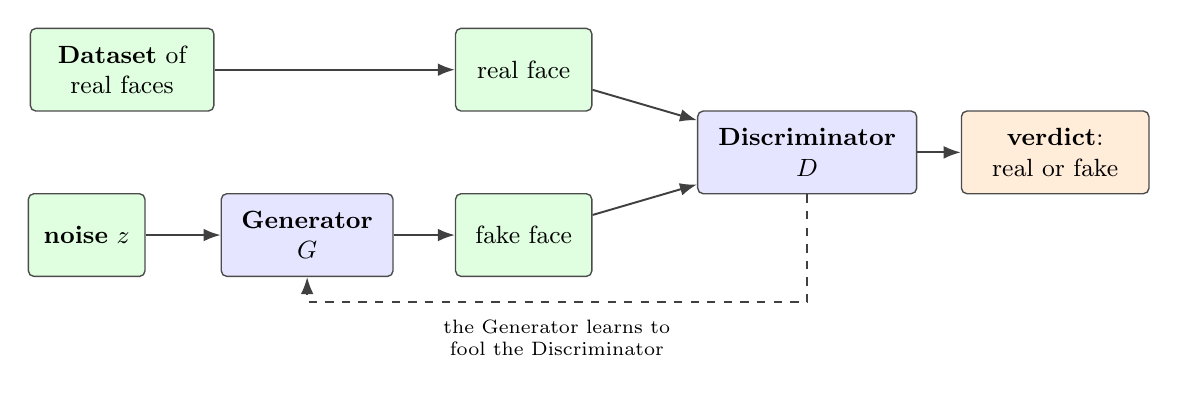
\begin{tikzpicture}[
    x=1cm, y=1cm,
    font=\small,
    block/.style={rectangle, rounded corners=2pt, draw=black!70, line width=0.5pt,
      fill=blue!10, align=center, inner sep=4pt, minimum height=9mm},
    inputblock/.style={block, fill=green!12},
    stageblock/.style={block, fill=orange!15},
    flow/.style={->, >=Latex, line width=0.7pt, draw=black!75},
    feed/.style={->, >=Latex, line width=0.7pt, draw=black!75, dashed},
  ]

  % ---------------- the data ----------------
  \node[inputblock, text width=1.20cm, minimum height=1.05cm] (z) at (0.75,0)
    {\textbf{noise} $z$};
  \node[inputblock, text width=2.05cm, minimum height=1.05cm] (data) at (1.20,2.10)
    {\textbf{Dataset} of\\real faces};
  \node[inputblock, text width=1.45cm, minimum height=1.05cm] (real) at (6.30,2.10)
    {real face};

  % ---------------- the two networks ----------------
  \node[block, text width=1.90cm, minimum height=1.05cm] (G) at (3.55,0)
    {\textbf{Generator}\\$G$};
  \node[block, text width=2.50cm, minimum height=1.05cm] (D) at (9.90,1.05)
    {\textbf{Discriminator}\\$D$};

  % ---------------- the fake face and the verdict ----------------
  \node[inputblock, text width=1.45cm, minimum height=1.05cm] (fake) at (6.30,0)
    {fake face};
  \node[stageblock, text width=2.10cm, minimum height=1.05cm] (verdict) at (13.05,1.05)
    {\textbf{verdict}:\\real or fake};

  % ---------------- arrows ----------------
  \draw[flow] (z) -- (G);
  \draw[flow] (G) -- (fake);
  \draw[flow] (data) -- (real);
  \draw[flow] (fake) -- (D);
  \draw[flow] (real) -- (D);
  \draw[flow] (D) -- (verdict);

  % ---------------- the training feedback ----------------
  \draw[feed] (D.south) -- (9.90,-0.85) -- (3.55,-0.85) -- (G.south);
  \node[font=\scriptsize, align=center, anchor=north] at (6.72,-0.95)
    {the Generator learns to\\fool the Discriminator};

  \end{tikzpicture}
  \caption{The training loop of a standard GAN. The Discriminator compares each
    fake face with real faces and gives a verdict; the dashed feedback teaches
    the Generator to fool it.}
  \label{fig:gan_training}
\end{figure}


\subsection{First Order Motion Model}
FOMM animates one source photo with the head motion and the facial expressions
from a driving video. The method comes from Siarohin et al. (``First Order
Motion Model for Image Animation'', NeurIPS 2019). It needs no landmark detector
and no 3D face model.
It learns its own keypoints per object category; our category is faces. It
follows Monkey-Net, which the paper calls the first object-agnostic deep model,
and FOMM improves on it.

\subsubsection{First-order motion}
0th order motion moves a point only in $x$ and $y$, so the skin keeps its
shape and the result looks stiff and robotic. 1st order motion also measures how
the skin around the point turns, grows and stretches, through a small
$2\times2$ Jacobian matrix per keypoint. The paper calls it a first order Taylor
expansion.

\subsubsection{The three parts}
The pipeline has three parts (Figure~\ref{fig:fomm_pipeline}).

% Figure: the First Order Motion Model pipeline (Siarohin et al., NeurIPS 2019).
% The keypoint detector reads the source image once and each driving frame.
% The dense motion network makes a motion field and an occlusion map.
% The generator warps the source features and inpaints the occluded parts.
% Requires in the preamble: \usepackage{tikz} + \usetikzlibrary{arrows.meta}
\begin{figure}[tb]
  \centering
  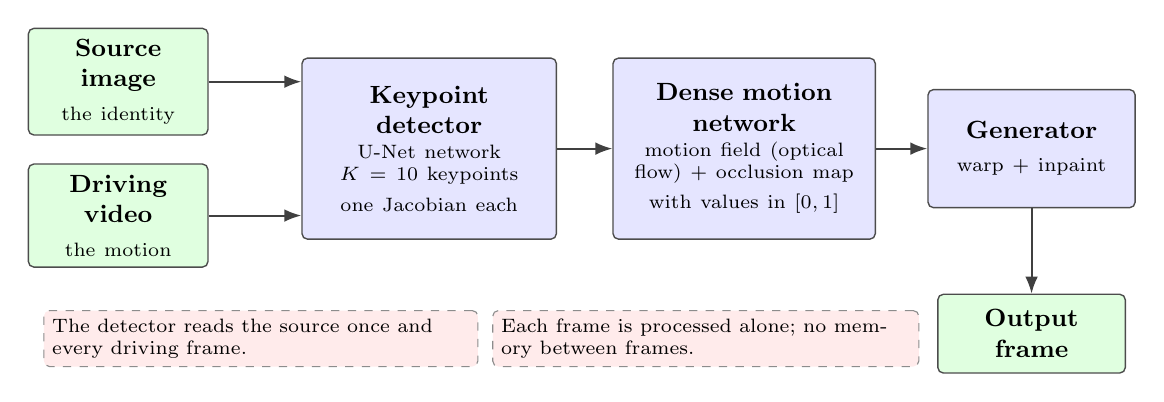
\begin{tikzpicture}[
    x=1cm, y=1cm,
    font=\small,
    block/.style={rectangle, rounded corners=2pt, draw=black!70, line width=0.5pt,
      fill=blue!10, align=center, inner sep=4pt, minimum height=9mm},
    inputblock/.style={block, fill=green!12},
    noteblock/.style={rectangle, rounded corners=2pt, draw=black!45, dashed,
      fill=red!8, align=left, inner sep=3pt, font=\scriptsize},
    flow/.style={->, >=Latex, line width=0.7pt, draw=black!75},
  ]

  % ---------------- inputs (left) ----------------
  \node[inputblock, text width=2.00cm, minimum height=1.10cm] (src) at (1.15,1.60)
    {\textbf{Source image}\\[1pt]\scriptsize the identity};
  \node[inputblock, text width=2.00cm, minimum height=1.10cm] (drv) at (1.15,-0.10)
    {\textbf{Driving video}\\[1pt]\scriptsize the motion};

  % ---------------- the three parts ----------------
  \node[block, text width=2.95cm, minimum height=2.30cm] (kpd) at (5.10,0.75)
    {\textbf{Keypoint detector}\\[1pt]\scriptsize U-Net network\\$K=10$ keypoints\\one Jacobian each};
  \node[block, text width=3.05cm, minimum height=2.30cm] (dmn) at (9.10,0.75)
    {\textbf{Dense motion}\\\textbf{network}\\[1pt]\scriptsize motion field (optical\\flow) + occlusion map\\with values in $[0,1]$};
  \node[block, text width=2.35cm, minimum height=1.50cm] (gen) at (12.75,0.75)
    {\textbf{Generator}\\[1pt]\scriptsize warp + inpaint};

  % ---------------- output ----------------
  \node[inputblock, text width=2.10cm, minimum height=1.00cm] (out) at (12.75,-1.60)
    {\textbf{Output frame}};

  % ---------------- arrows ----------------
  \draw[flow] (src.east) -- (kpd.west |- src.east);
  \draw[flow] (drv.east) -- (kpd.west |- drv.east);
  \draw[flow] (kpd) -- (dmn);
  \draw[flow] (dmn) -- (gen);
  \draw[flow] (gen.south) -- (out.north);

  % ---------------- notes ----------------
  \node[noteblock, text width=5.30cm, anchor=north west] at (0.20,-1.30)
    {The detector reads the source once and every driving frame.};
  \node[noteblock, text width=5.20cm, anchor=north west] at (5.90,-1.30)
    {Each frame is processed alone; no memory between frames.};

  \end{tikzpicture}
  \caption{The First Order Motion Model pipeline: keypoints with Jacobians, a
    motion field and an occlusion map, then warp and inpaint. Each frame is
    processed alone.}
  \label{fig:fomm_pipeline}
\end{figure}


The \textbf{keypoint detector} is a U-Net network (the paper's word; the code
names the class Hourglass). It finds $K=10$ keypoints for the faces model and
one Jacobian per keypoint. The expected point position is a weighted average
over the output heatmaps (soft-argmax). An equivariance loss teaches the
detector during training, so it needs no keypoint labels.

The \textbf{dense motion network} turns the sparse keypoints into a dense motion
field (optical flow) and an occlusion map with values between 0 and 1.

The \textbf{generator} warps the source features with the flow. The code
multiplies the warped features by the occlusion map
(\texttt{out = out * occlusion\_map}). Where the map is near 0, the warped
pixels lose their weight and the decoder fills the area from learned face priors
(inpainting).

Each frame is processed on its own. No state passes from frame to frame (no
recurrence).

\subsubsection{Occlusion and inpainting}
A closed mouth or a turned head reveals pixels that do not exist in the source
photo (self-occlusion). Where $O$ is near 1, the pixels come from the source.
Where $O$ is near 0, the network draws the area itself from the training-set
average (Figure~\ref{fig:fomm_occlusion}).

These are the failure modes we saw. Rare personal details are lost in inpainted
areas. Very large head turns, about 45 degrees or more, leave blurry patches.
Both limits come from our own observation, not from the paper.

% Figure: occlusion and inpainting in the FOMM generator.
% A closed mouth or a turned head reveals pixels that are missing in the source.
% $O \approx 1$: the pixels come from the source. $O \approx 0$: the network
% draws the area itself from the training-set average.
% Requires in the preamble: \usepackage{tikz} + \usetikzlibrary{arrows.meta}
\begin{figure}[tb]
  \centering
  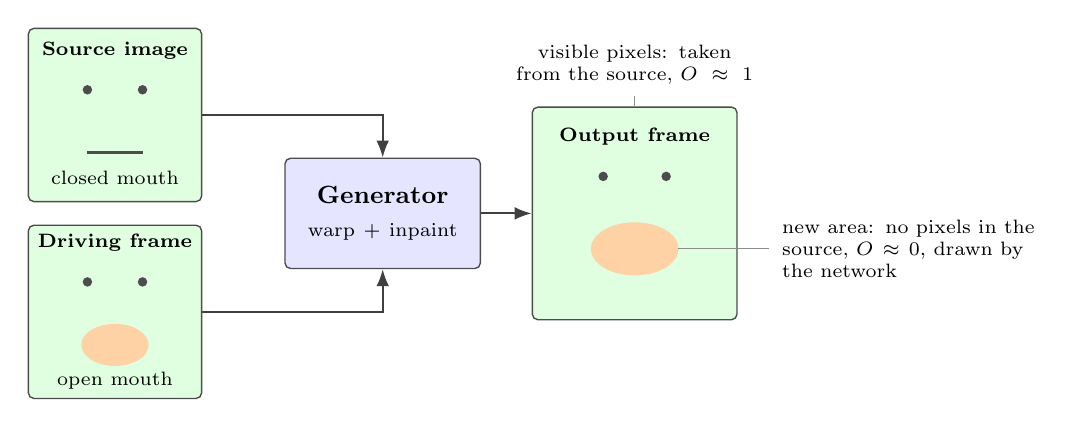
\begin{tikzpicture}[
    x=1cm, y=1cm,
    font=\small,
    block/.style={rectangle, rounded corners=2pt, draw=black!70, line width=0.5pt,
      fill=blue!10, align=center, inner sep=4pt, minimum height=9mm},
    inputblock/.style={block, fill=green!12},
    flow/.style={->, >=Latex, line width=0.7pt, draw=black!75},
    leader/.style={draw=black!45, line width=0.4pt},
  ]

  % ---------------- source frame (closed mouth) ----------------
  \node[inputblock, minimum width=2.20cm, minimum height=2.20cm] (src) at (1.15,0.90) {};
  \node[font=\scriptsize] at (1.15,1.72) {\textbf{Source image}};
  \fill[black!70] (0.80,1.22) circle (0.6mm);
  \fill[black!70] (1.50,1.22) circle (0.6mm);
  \draw[black!70, line width=1pt] (0.80,0.42) -- (1.50,0.42);
  \node[font=\scriptsize] at (1.15,0.10) {closed mouth};

  % ---------------- driving frame (open mouth) ----------------
  \node[inputblock, minimum width=2.20cm, minimum height=2.20cm] (drv) at (1.15,-1.60) {};
  \node[font=\scriptsize] at (1.15,-0.72) {\textbf{Driving frame}};
  \fill[black!70] (0.80,-1.22) circle (0.6mm);
  \fill[black!70] (1.50,-1.22) circle (0.6mm);
  \fill[draw=black!60, line width=0.4pt, orange!35] (1.15,-2.02) ellipse (0.42cm and 0.26cm);
  \node[font=\scriptsize] at (1.15,-2.47) {open mouth};

  % ---------------- generator ----------------
  \node[block, text width=2.20cm, minimum height=1.40cm] (gen) at (4.55,-0.35)
    {\textbf{Generator}\\[1pt]\scriptsize warp + inpaint};
  \draw[flow] (src.east) -| (gen.north);
  \draw[flow] (drv.east) -| (gen.south);

  % ---------------- output frame ----------------
  \node[inputblock, minimum width=2.60cm, minimum height=2.70cm] (out) at (7.75,-0.35) {};
  \node[font=\scriptsize] at (7.75,0.62) {\textbf{Output frame}};
  \fill[black!70] (7.35,0.12) circle (0.6mm);
  \fill[black!70] (8.15,0.12) circle (0.6mm);
  \fill[draw=black!60, line width=0.4pt, orange!35] (7.75,-0.80) ellipse (0.55cm and 0.33cm);
  \draw[flow] (gen.east) -- (out.west);

  % ---------------- the two regions ----------------
  \draw[leader] (7.75,1.00) -- (7.75,1.14);
  \node[font=\scriptsize, align=center, text width=4.30cm, anchor=south]
    at (7.75,1.16) {visible pixels: taken from the source, $O\approx1$};
  \draw[leader] (8.30,-0.80) -- (9.45,-0.80);
  \node[font=\scriptsize, align=left, text width=3.30cm, anchor=west]
    at (9.50,-0.80) {new area: no pixels in the source, $O\approx0$, drawn by the network};

  \end{tikzpicture}
  \caption{Occlusion and inpainting. Where $O$ is near 1, the pixels come from
    the source. Where $O$ is near 0, the network draws the missing pixels
    itself.}
  \label{fig:fomm_occlusion}
\end{figure}


\subsection{Local experiment}
We ran the released VoxCeleb checkpoint \texttt{vox-cpk.pth.tar} in CPU mode on
an Apple Silicon machine. The source portrait is 512x512; the driving clip is
256x256, 320 frames, 29.97 FPS. With \texttt{-{}-relative} the keypoints move
relative to the first frame; \texttt{-{}-adapt\_scale} adjusts the motion size
with the convex hull of the keypoints.

The output is 256x256, 320 frames, 29.97 FPS and 10.7 seconds long. The recorded
speed is about 2.05 iterations per second, about 2.5 minutes in total. Head
turns and blinks transferred smoothly; mouth motion needed inpainting.
Table~\ref{tab:fomm_run} lists the setup and the output.

\begin{table}[tb]
  \centering
  \footnotesize
  \begin{tabular}{@{}l l@{}}
    \toprule
    Item & Value \\
    \midrule
    Checkpoint & \texttt{vox-cpk.pth.tar} (VoxCeleb) \\
    Source portrait & 512 $\times$ 512 \\
    Driving clip & 256 $\times$ 256, 320 frames, 29.97 FPS \\
    Mode and flags & CPU, \texttt{-{}-relative}, \texttt{-{}-adapt\_scale} \\
    Output & 256 $\times$ 256, 320 frames, 29.97 FPS, 10.7 s \\
    Speed & about 2.05 it/s, about 2.5 minutes \\
    \bottomrule
  \end{tabular}
  \caption{The local FOMM run: setup, flags and output.}
  \label{tab:fomm_run}
\end{table}

\subsection{Failure mode: braces}
The VoxCeleb training data has no braces, so the mouth area should lose them
when inpainting starts. Our frames confirm this (Table~\ref{tab:fomm_braces}).

\begin{table}[tb]
  \centering
  \footnotesize
  \begin{tabular}{@{}r r l l@{}}
    \toprule
    Frame & Time & Driving mouth & Active path and result \\
    \midrule
    10 & 0.3 s & small shift & warping, $O\approx1$: braces kept \\
    195 & 6.5 s & lips close & mouth hidden \\
    288 & 9.6 s & wide smile & inpainting, $O\approx0$: plain teeth \\
    \bottomrule
  \end{tabular}
  \caption{The braces test: the active path decides where the mouth pixels come
    from.}
  \label{tab:fomm_braces}
\end{table}

The active path decides which pixels appear: warped areas keep the pixels of the
person, and inpainted areas follow the training data. FOMM gave the project a
fast per-frame method. Identity details survive only in warped areas, and rare
details such as braces are lost as soon as inpainting starts. There is no memory
across frames, so the method cannot repair a frame from its neighbours.

% Section 4: rectified flow head swap with FLUX.2-klein-4B.
% Numbers come from the run artifacts rectified_flow/final_report/faceswap_20_metrics_summary.csv
% and rectified_flow/final_report/REPORT.md; these artifacts are not in the repository.
% Figure inputs are relative to docs/report/.

\section{Rectified Flow Head Swap}

\subsection{Scope and hardware}
We wanted to swap a video face with one from a selfie. The run had to stay on one laptop with a 4 GB NVIDIA GPU and 8 GB of system RAM. We sent no data to a cloud service.

The output had to keep the source motion, expression, lighting and background. Only the head should change. The clip is 96 frames at 512x512 and lasts 3.2 seconds.

\subsection{How we measured}
Every number comes from one script, run once per variant, each on the same 96 frames (175 to 270). The results table reports it. The raw run records, the metric CSV and the 96-frame sets are not in the repository, so the reported numbers cannot be re-derived from this checkout.

Face change is a temporal change indicator: the mean absolute grey difference between two frames inside one face box. The code takes the box from the first frame of the pair and reuses it for the second frame, so the box is not aligned to the second frame. Motion, lighting, texture change and flicker all enter the value, and the value has no calibrated threshold. The unswapped footage sets the control level.

Consecutive identity is how similar a face is to the one before it, measured in a face recognition embedding, so a high value means temporal similarity; a wrong identity that stays consistent also scores high. Identity to the portrait measures similarity to the reference portrait; the unswapped footage scores near zero because it is a different person. Hair noise is how much the hair region flickers, and lower is better; p95 marks the worst frames, the value 95 percent stay under.

\subsection{Pipeline overview}
The flow has four stages. Generation transfers the identity, restoration cleans each face with GFPGAN, smoothing removes the boil, and reassembly attaches the audio. Only the last stage writes a video file.

The boil is the flicker that comes from generating each frame on its own. Figure~\ref{fig:pipeline_overview} shows the chain in order, with the cost of each stage.

% Figure: pipeline overview of the face-reenactment flow (four stages).
% Facts and numbers come from diffusion/REPORT.md.
% Requires in the preamble: \usepackage{tikz} + \usetikzlibrary{arrows.meta}
\begin{figure}[t]
  \centering
  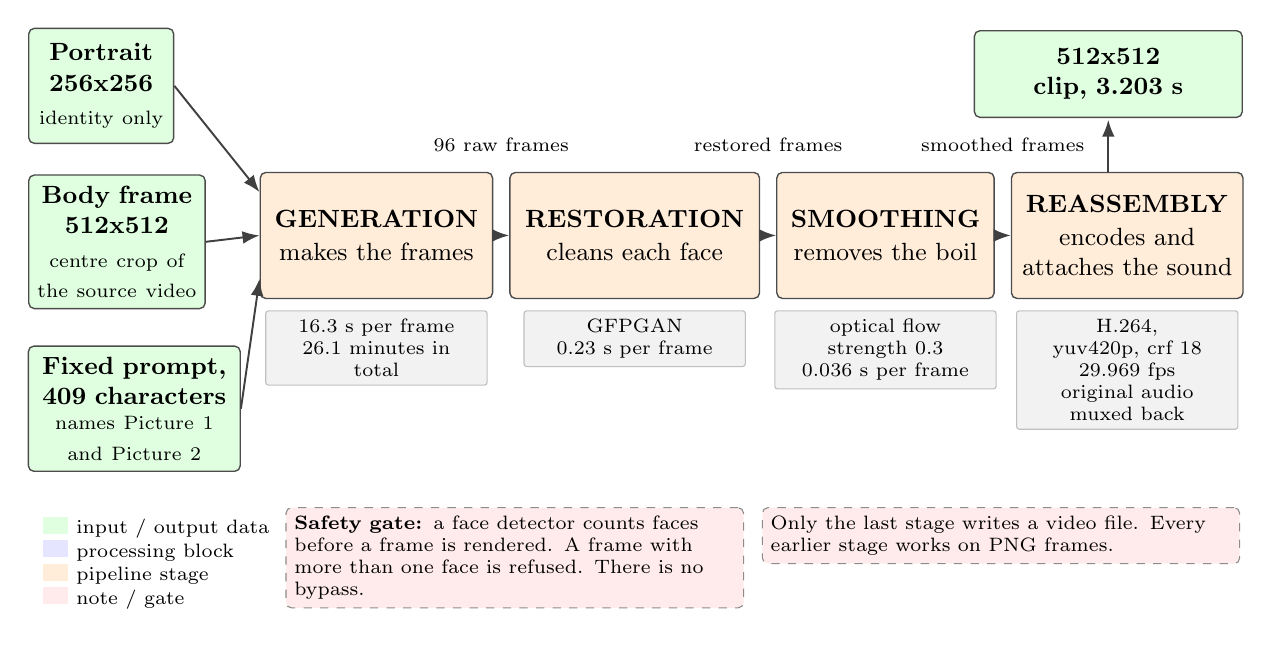
\begin{tikzpicture}[
    x=1cm, y=1cm,
    font=\small,
    block/.style={rectangle, rounded corners=2pt, draw=black!70, line width=0.5pt,
      fill=blue!10, align=center, inner sep=4pt, minimum height=9mm},
    inputblock/.style={rectangle, rounded corners=2pt, draw=black!70, line width=0.5pt,
      fill=green!12, align=center, inner sep=4pt, minimum height=9mm},
    stageblock/.style={rectangle, rounded corners=2pt, draw=black!70, line width=0.5pt,
      fill=orange!15, align=center, inner sep=4pt, minimum height=9mm},
    noteblock/.style={rectangle, rounded corners=2pt, draw=black!45, dashed,
      fill=red!8, align=left, inner sep=3pt, font=\scriptsize},
    flow/.style={->, >=Latex, line width=0.7pt, draw=black!75},
    arrowlab/.style={font=\scriptsize, fill=white, inner sep=1pt},
    cost/.style={draw=black!25, rounded corners=1pt, fill=gray!10, align=center,
      inner sep=3pt, font=\scriptsize, text width=2.6cm},
  ]

  % ---------------- inputs (left) ----------------
  \node[inputblock, inner xsep=2pt, text width=1.70cm, minimum height=1.46cm] (inP) at (0.96,1.90)
    {\textbf{Portrait}\\\textbf{256x256}\\[1pt]\scriptsize identity only};
  \node[inputblock, inner xsep=2pt, text width=2.10cm] (inB) at (1.16,-0.0806)
    {\textbf{Body frame}\\\textbf{512x512}\\[1pt]\scriptsize centre crop of
     the source video};
  \node[inputblock, inner xsep=2pt, text width=2.55cm] (inF) at (1.38,-2.20)
    {\textbf{Fixed prompt,}\\\textbf{409 characters}\\[1pt]\scriptsize names Picture 1\\and Picture 2};

  % ---------------- four stages (left to right) ----------------
  \node[stageblock, inner xsep=2pt, text width=2.81cm, minimum height=1.60cm] (S1) at (4.455,0)
    {\textbf{GENERATION}\\[1pt] makes the frames};
  \node[stageblock, inner xsep=2pt, text width=3.03cm, minimum height=1.60cm] (S2) at (7.735,0)
    {\textbf{RESTORATION}\\[1pt] cleans each face};
  \node[stageblock, inner xsep=2pt, text width=2.62cm, minimum height=1.60cm] (S3) at (10.920,0)
    {\textbf{SMOOTHING}\\[1pt] removes the boil};
  \node[stageblock, inner xsep=2pt, text width=2.80cm, minimum height=1.60cm] (S4) at (13.990,0)
    {\textbf{REASSEMBLY}\\[1pt] encodes and\\attaches the sound};

  % ---------------- input arrows into stage 1 ----------------
  \draw[flow] (inP.east) -- (S1.west |- 0,0.55);
  \draw[flow] (inB.east) -- (S1.west);
  \draw[flow] (inF.east) -- (S1.west |- 0,-0.55);

  % ---------------- data between the stages ----------------
  \draw[flow] (S1.east) -- (S2.west);
  \draw[flow] (S2.east) -- (S3.west);
  \draw[flow] (S3.east) -- (S4.west);
  \node[arrowlab] at (6.04,1.15) {96 raw frames};
  \node[arrowlab] at (9.43,1.15) {restored frames};
  \node[arrowlab] at (12.41,1.15) {smoothed frames};

  % ---------------- final output ----------------
  \node[inputblock, text width=3.12cm, minimum height=1.10cm] (out) at (13.75,2.05)
    {\textbf{512x512 clip, 3.203 s}};
  \draw[flow] (S4.north -| 13.75,0) -- (13.75,1.47);

  % ---------------- per-stage cost lines ----------------
  \node[cost, anchor=north] at (4.455,-0.95)
    {16.3 s per frame\\26.1 minutes in\\total};
  \node[cost, anchor=north] at (7.735,-0.95)
    {GFPGAN\\0.23 s per frame};
  \node[cost, anchor=north] at (10.920,-0.95)
    {optical flow\\strength 0.3\\0.036 s per frame};
  \node[cost, anchor=north] at (13.990,-0.95)
    {H.264, yuv420p, crf 18\\29.969 fps\\original audio muxed back};

  % ---------------- notes ----------------
  \node[noteblock, execute at begin node=\raggedright, text width=5.60cm, anchor=north west] at (3.30,-3.45)
    {\textbf{Safety gate:} a face detector counts faces before a frame is
     rendered. A frame with more than one face is refused. There is no bypass.};
  \node[noteblock, execute at begin node=\raggedright, text width=5.85cm, anchor=north west] at (9.35,-3.45)
    {Only the last stage writes a video file. Every earlier stage works on PNG frames.};

  % ---------------- legend ----------------
  \node[font=\scriptsize, anchor=north west] (leg) at (0.10,-3.45)
    {\begin{tabular}{@{}c@{\hspace{3pt}}l@{}}
       \tikz\fill[draw=black!70,line width=0.4pt,green!12] (0,0) rectangle (0.30,0.20); & input / output data\\
       \tikz\fill[draw=black!70,line width=0.4pt,blue!10]  (0,0) rectangle (0.30,0.20); & processing block\\
       \tikz\fill[draw=black!70,line width=0.4pt,orange!15](0,0) rectangle (0.30,0.20); & pipeline stage\\
       \tikz\fill[draw=black!45,line width=0.4pt,red!8]    (0,0) rectangle (0.30,0.20); & note / gate\\
     \end{tabular}};

  \end{tikzpicture}
  \caption{The four-stage pipeline: generation, restoration, smoothing and
    reassembly, with the cost measured for each stage.}
  \label{fig:pipeline_overview}
\end{figure}

\subsection{How a rectified flow model works}
A rectified flow model learns one job: connect a clean image and noise with a straight line. Training picks one random time per example and mixes the two ends at that time. The model predicts the direction that points from the noise end to the image end. The guess is compared with the true direction along the line, and the weights are then nudged.

At sampling time the same model starts from pure noise. Each Euler step moves the sample a small way along the predicted direction, and an image forms. The sampling code calls these steps denoising steps, because the sample becomes less noisy at each step. Figure~\ref{fig:rectified_flow_process} draws training and sampling side by side.

We did not train the base model; we used a released checkpoint. The released model is step distilled, so four steps are enough for it. We could not tell the difference between four steps and eight.

% Figure: the rectified flow model, in training and at sampling.
% Training mixes an image and noise at one random time on a straight line;
% sampling takes four Euler steps along the predicted direction.
% Facts come from the published model repository and model card.
% Requires in the preamble: \usepackage{tikz} + \usetikzlibrary{positioning,arrows.meta}
\begin{figure}[t]
  \centering
  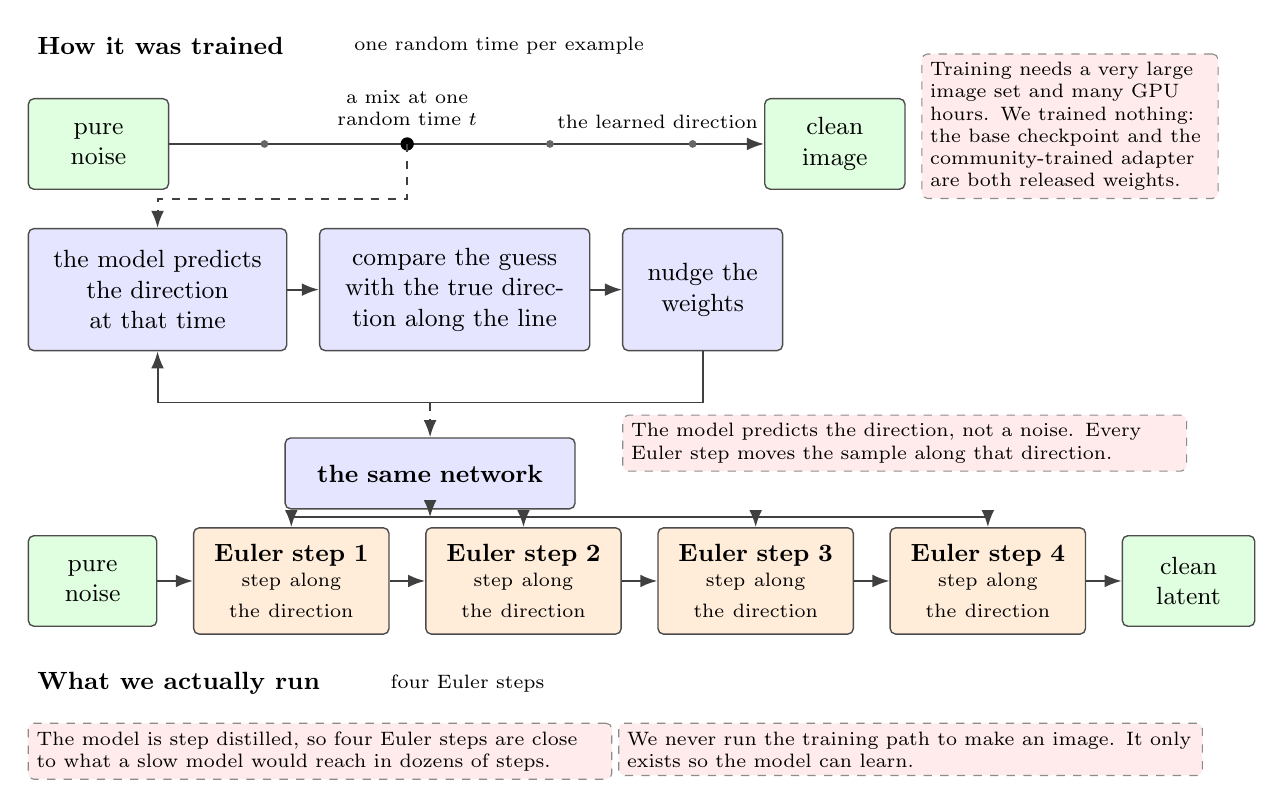
\begin{tikzpicture}[
    x=1cm, y=1cm,
    font=\small,
    block/.style={rectangle, rounded corners=2pt, draw=black!70, line width=0.5pt,
      fill=blue!10, align=center, inner sep=4pt, minimum height=9mm},
    inputblock/.style={block, fill=green!12},
    stageblock/.style={block, fill=orange!15},
    noteblock/.style={rectangle, rounded corners=2pt, draw=black!45, dashed,
      fill=red!8, align=left, inner sep=3pt, font=\scriptsize},
    flow/.style={->, >=Latex, line width=0.7pt, draw=black!75},
    feed/.style={->, >=Latex, line width=0.7pt, draw=black!75, dashed},
    arrowlab/.style={font=\scriptsize, fill=white, inner sep=1pt},
  ]

  % ================= top half: how it was trained =================
  \node[anchor=west] (headT) at (0.15,10.45) {\textbf{How it was trained}};
  \node[font=\scriptsize, anchor=west, right=0.65cm of headT] (dirT)
    {one random time per example};

  % one straight line between the noise end and the image end
  \node[inputblock, anchor=west, text width=1.50cm, minimum height=1.15cm] (noiseT) at (0.15,9.20)
    {pure\\noise};
  \node[inputblock, anchor=east, text width=1.50cm, minimum height=1.15cm] (imageT) at (11.30,9.20)
    {clean\\image};
  \draw[flow] (noiseT.east) -- (imageT.west)
    coordinate[pos=0.16] (tp1) coordinate[pos=0.40] (tp2)
    coordinate[pos=0.64] (tp3) coordinate[pos=0.88] (tp4);
  \foreach \p in {tp1,tp3,tp4}{\fill[black!60] (\p) circle (1.4pt);}
  \fill[black] (tp2) circle (2.4pt);
  \node[font=\scriptsize, align=center, anchor=south] at ([yshift=3pt]tp2)
    {a mix at one\\random time $t$};
  \node[font=\scriptsize, anchor=south] at (8.15,9.27) {the learned direction};

  % the training loop: predict, compare, nudge, repeat
  \node[block, anchor=west, text width=3.00cm, minimum height=1.55cm] (lt1) at (0.15,7.35)
    {the model predicts the direction at that time};
  \node[block, text width=3.15cm, minimum height=1.55cm, right=0.40cm of lt1] (lt2)
    {compare the guess with the true direction along the line};
  \node[block, text width=1.75cm, minimum height=1.55cm, right=0.40cm of lt2] (lt3)
    {nudge the weights};
  \draw[feed] (tp2) -- ++(0,-0.70) -| (lt1.north);
  \draw[flow] (lt1) -- (lt2);
  \draw[flow] (lt2) -- (lt3);
  \draw[flow] (lt3.south) -- ++(0,-0.65) coordinate (retcT) -- (retcT -| lt1.south) -- (lt1.south);

  % ---------------- the one box that both halves use ----------------
  \path (lt1.center) -- (lt3.center) coordinate[midway] (loopmidT);
  \coordinate (retmidT) at (loopmidT |- retcT);
  \node[block, text width=3.40cm, minimum height=0.90cm] (net) at ([yshift=-0.90cm]retmidT)
    {\textbf{the same network}};
  \draw[feed] (retmidT) -- (net.north);

  % ================= bottom half: what we actually run =================
  \node[inputblock, anchor=west, text width=1.35cm, minimum height=1.15cm] (noiseB) at (0.15,3.65)
    {pure\\noise};
  \node[stageblock, text width=2.20cm, minimum height=1.35cm, right=0.45cm of noiseB] (st1)
    {\textbf{Euler step 1}\\[1pt]\scriptsize step along\\the direction};
  \node[stageblock, text width=2.20cm, minimum height=1.35cm, right=0.45cm of st1] (st2)
    {\textbf{Euler step 2}\\[1pt]\scriptsize step along\\the direction};
  \node[stageblock, text width=2.20cm, minimum height=1.35cm, right=0.45cm of st2] (st3)
    {\textbf{Euler step 3}\\[1pt]\scriptsize step along\\the direction};
  \node[stageblock, text width=2.20cm, minimum height=1.35cm, right=0.45cm of st3] (st4)
    {\textbf{Euler step 4}\\[1pt]\scriptsize step along\\the direction};
  \node[inputblock, text width=1.40cm, minimum height=1.15cm, right=0.45cm of st4] (latentB)
    {clean\\latent};
  \draw[flow] (noiseB) -- (st1);
  \draw[flow] (st1) -- (st2);
  \draw[flow] (st2) -- (st3);
  \draw[flow] (st3) -- (st4);
  \draw[flow] (st4) -- (latentB);

  % the same network drives every Euler step
  \coordinate (busY) at (0,4.46);
  \draw[flow] (net.south) -- (net.south |- busY);
  \draw[draw=black!75, line width=0.7pt] (st1.north |- busY) -- (st4.north |- busY);
  \foreach \s in {st1,st2,st3,st4}{\draw[flow] (\s.north |- busY) -- (\s.north);}

  \node[anchor=west] (headB) at (0.15,2.35) {\textbf{What we actually run}};
  \node[font=\scriptsize, anchor=west, right=0.65cm of headB] (dirB) {four Euler steps};

  % ================= notes =================
  \node[noteblock, text width=3.55cm, anchor=north west] at (11.50,10.35)
    {Training needs a very large image set and many GPU hours. We trained nothing: the
     base checkpoint and the community-trained adapter are both released weights.};
  \node[noteblock, text width=6.95cm, anchor=west] at (7.70,5.40)
    {The model predicts the direction, not a noise. Every Euler step moves the sample
     along that direction.};
  \node[noteblock, text width=7.20cm, anchor=north west] at (0.15,1.85)
    {The model is step distilled, so four Euler steps are close to what a slow model would
     reach in dozens of steps.};
  \node[noteblock, text width=7.20cm, anchor=north west] at (7.65,1.85)
    {We never run the training path to make an image. It only exists so the model can learn.};

  \end{tikzpicture}
  \caption{The rectified flow model in training and at sampling. Training draws one random
    time per example, mixes the image and noise at that time, and teaches the model the
    direction along the straight line between the two ends. Sampling starts from noise and
    takes four Euler steps along the predicted direction. Both jobs use one and the same
    network.}
  \label{fig:rectified_flow_process}
\end{figure}

\subsection{The model and the LoRA adapter}
The model is a stack of transformer blocks (Figure~\ref{fig:architecture_lora}). A latent token of 128 channels is projected to width 3072. It passes through five double-stream blocks, then 20 single-stream blocks and a final layer. In the first part the text and image tokens stay apart, and they meet through joint attention.

Later the two streams are joined into one. The final layer projects back to 128 channels for the decoder.

The adapter is a small pair of matrices, A and B, trained beside each frozen weight. The adapter attaches inside the transformer blocks. It takes the attention projections and the feed-forward linears, and in the single-stream blocks the two fused linears. The block output adds a scaled product of A and B to the frozen term. Only A and B are trained, so the base weights never change. The adapter carries the head swap behaviour.

% Figure: the denoiser drawn as a stack of layers, and the LoRA adapter on one linear layer.
% Facts come from the published model repository and model card.
% Requires in the preamble: \usepackage{tikz} + \usetikzlibrary{positioning,arrows.meta},
%                            and amsmath for \frac in the adapter formula.
\begin{figure}[t]
  \centering
  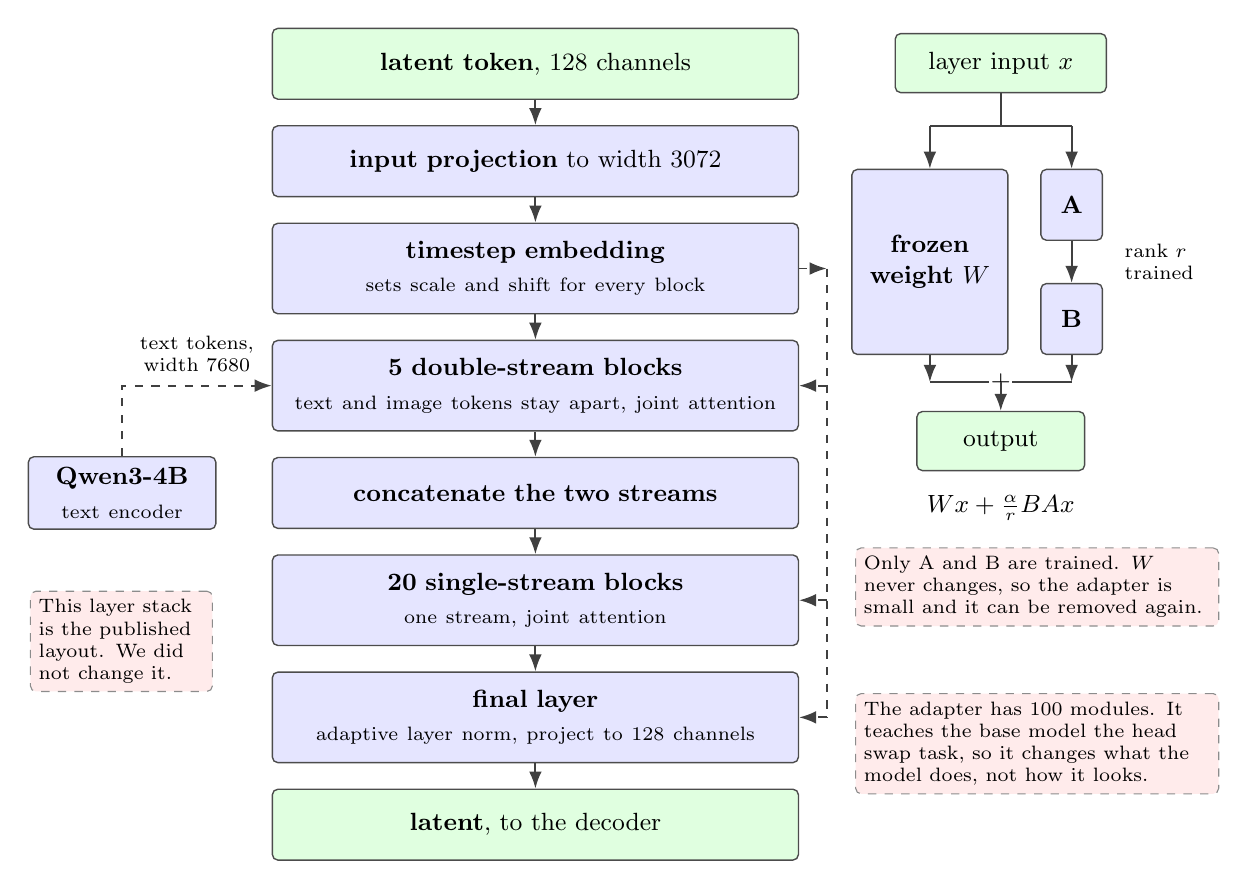
\begin{tikzpicture}[
    x=1cm, y=1cm,
    font=\small,
    block/.style={rectangle, rounded corners=2pt, draw=black!70, line width=0.5pt,
      fill=blue!10, align=center, inner sep=4pt, minimum height=9mm},
    inputblock/.style={block, fill=green!12},
    stageblock/.style={block, fill=orange!15},
    noteblock/.style={rectangle, rounded corners=2pt, draw=black!45, dashed,
      fill=red!8, align=left, inner sep=3pt, font=\scriptsize},
    flow/.style={->, >=Latex, line width=0.7pt, draw=black!75},
    feed/.style={->, >=Latex, line width=0.7pt, draw=black!75, dashed},
    arrowlab/.style={font=\scriptsize, fill=white, inner sep=1pt},
  ]

  % ================= left part: the denoiser as a stack of layers =================
  \node[inputblock, anchor=north, text width=6.40cm, minimum height=0.90cm] (lat) at (6.54,10.55)
    {\textbf{latent token}, 128 channels};
  \node[block, text width=6.40cm, minimum height=0.90cm, below=0.32cm of lat] (proj)
    {\textbf{input projection} to width 3072};
  \node[block, text width=6.40cm, minimum height=1.15cm, below=0.32cm of proj] (tstep)
    {\textbf{timestep embedding}\\[1pt]\scriptsize sets scale and shift for every block};
  \node[block, text width=6.40cm, minimum height=1.15cm, below=0.32cm of tstep] (ds)
    {\textbf{5 double-stream blocks}\\[1pt]\scriptsize text and image tokens stay apart,
     joint attention};
  \node[block, text width=6.40cm, minimum height=0.90cm, below=0.32cm of ds] (cat)
    {\textbf{concatenate the two streams}};
  \node[block, text width=6.40cm, minimum height=1.15cm, below=0.32cm of cat] (ss)
    {\textbf{20 single-stream blocks}\\[1pt]\scriptsize one stream, joint attention};
  \node[block, text width=6.40cm, minimum height=1.15cm, below=0.32cm of ss] (fin)
    {\textbf{final layer}\\[1pt]\scriptsize adaptive layer norm, project to 128 channels};
  \node[inputblock, text width=6.40cm, minimum height=0.90cm, below=0.32cm of fin] (latout)
    {\textbf{latent}, to the decoder};
  \foreach \a/\b in {lat/proj, proj/tstep, tstep/ds, ds/cat, cat/ss, ss/fin, fin/latout}
    {\draw[flow] (\a.south) -- (\b.north);}

  % the text encoder enters through joint attention (dashed = conditioning path)
  \node[block, text width=2.10cm, left=0.70cm of cat] (enc)
    {\textbf{Qwen3-4B}\\[1pt]\scriptsize text encoder};
  \coordinate (txtcorner) at (enc.north |- ds.center);
  \draw[feed] (enc.north) -- (txtcorner) -- (ds.west);
  \path (txtcorner) -- (ds.west) coordinate[midway] (txtmid);
  \node[arrowlab, align=center, text width=1.70cm, anchor=south] at ([yshift=0.14cm]txtmid)
    {text tokens,\\width 7680};

  % the timestep embedding modulates every block (dashed = conditioning path)
  \draw[feed] (tstep.east) -- ++(0.35,0) coordinate (tbus);
  \draw[draw=black!75, line width=0.7pt, dashed] (tbus) -- (tbus |- fin.center);
  \foreach \s in {ds,ss,fin}{\draw[feed] (tbus |- \s.center) -- (\s.east);}

  % ================= right part: how the adapter attaches =================
  \node[inputblock, text width=2.40cm, minimum height=0.75cm] (layin) at (12.45,10.10)
    {layer input $x$};
  \node[block, text width=1.70cm, minimum height=2.35cm] (wgt) at (11.55,7.575)
    {\textbf{frozen weight $W$}};
  \node[block, text width=0.50cm, minimum height=0.90cm] (bA) at (13.35,8.30) {\textbf{A}};
  \node[block, text width=0.50cm, minimum height=0.90cm] (bB) at (13.35,6.85) {\textbf{B}};
  \draw[flow] (bA.south) -- (bB.north);

  \coordinate (br) at (12.45,9.30);
  \draw[draw=black!75, line width=0.7pt] (layin.south) -- (br);
  \draw[draw=black!75, line width=0.7pt] (br -| wgt.north) -- (br -| bA.north);
  \draw[flow] (br -| wgt.north) -- (wgt.north);
  \draw[flow] (br -| bA.north) -- (bA.north);

  \coordinate (mg) at (12.45,6.05);
  \draw[flow] (wgt.south) -- (mg -| wgt.south);
  \draw[flow] (bB.south) -- (mg -| bB.south);
  \draw[draw=black!75, line width=0.7pt] (mg -| wgt.south) -- (mg -| bB.south);
  \node[fill=white, inner sep=0.5pt] at (mg) {$+$};
  \node[inputblock, text width=1.85cm, minimum height=0.75cm] (layout) at (12.45,5.30)
    {output};
  \draw[flow] (mg) -- (layout.north);
  \node[font=\small] (formula) at (12.45,4.45) {$Wx + \frac{\alpha}{r}BAx$};

  \node[font=\scriptsize, align=left, text width=1.05cm, anchor=west] (abl) at (13.90,7.575)
    {rank $r$\\trained};

  % ================= notes =================
  \node[noteblock, text width=2.10cm, anchor=north west] at (0.12,3.40)
    {This layer stack is the published layout. We did not change it.};
  \node[noteblock, text width=4.40cm, anchor=north west] at (10.60,3.95)
    {Only A and B are trained. $W$ never changes, so the adapter is small and it can be
     removed again.};
  \node[noteblock, text width=4.40cm, anchor=north west] at (10.60,2.10)
    {The adapter has 100 modules. It teaches the base model the head swap task, so it changes
     what the model does, not how it looks.};

  \end{tikzpicture}
  \caption{The denoiser as a stack of layers. The text encoder and the timestep embedding enter
    as conditioning, and the adapter adds a small trained branch beside a frozen weight.}
  \label{fig:architecture_lora}
\end{figure}

\subsection{Generation}
Generation (Figure~\ref{fig:generation_architecture}) covers conditioning, sampling and decoding. A fixed prompt of 409 characters names Picture 1 as the body and Picture 2 as the head.

Qwen3-4B encodes the prompt once per session on the CPU, about 80 seconds, and its memory is then freed. Both pictures become VAE latents: the 512x512 body crop a 64x64x32 grid of about 1024 tokens, the 256x256 portrait about 256 tokens.

FLUX.2-klein-4B renders each frame in four sampling steps. Each step moves the latent along the direction the model predicts. The sampler calls the model once per step and feeds the result back. The text embeddings and the two image latents guide every step. A community-trained LoRA adapter of 80 adapted weights carries the head swap.

The same VAE decodes the final latent into pixels. Picture order is part of the adapter contract: the adapter's own documentation names Picture 1 the body and Picture 2 the head, and says not to reverse the images. A reversed order gives the wrong head.

The generator runs as a 4-bit GGUF file. The production loop calls the generator once per frame and holds no face gate, and no multi-face check exists on the generation path. The only face check sits in the restoration stage: the gate passes a frame only when it detects exactly one face. Frames with no face or with two or more faces are copied through unchanged.

The output is 96 frames from 5.8 to 9.0 seconds of the source, all with one fixed seed. Each frame took 16.3 seconds, so the stage used 26.1 minutes.

% Figure: architecture of the generation stage (conditioning, denoising, decoding).
% Facts and numbers come from diffusion/REPORT.md.
% Requires in the preamble: \usepackage{tikz} + \usetikzlibrary{arrows.meta}
\begin{figure}[t]
  \centering
  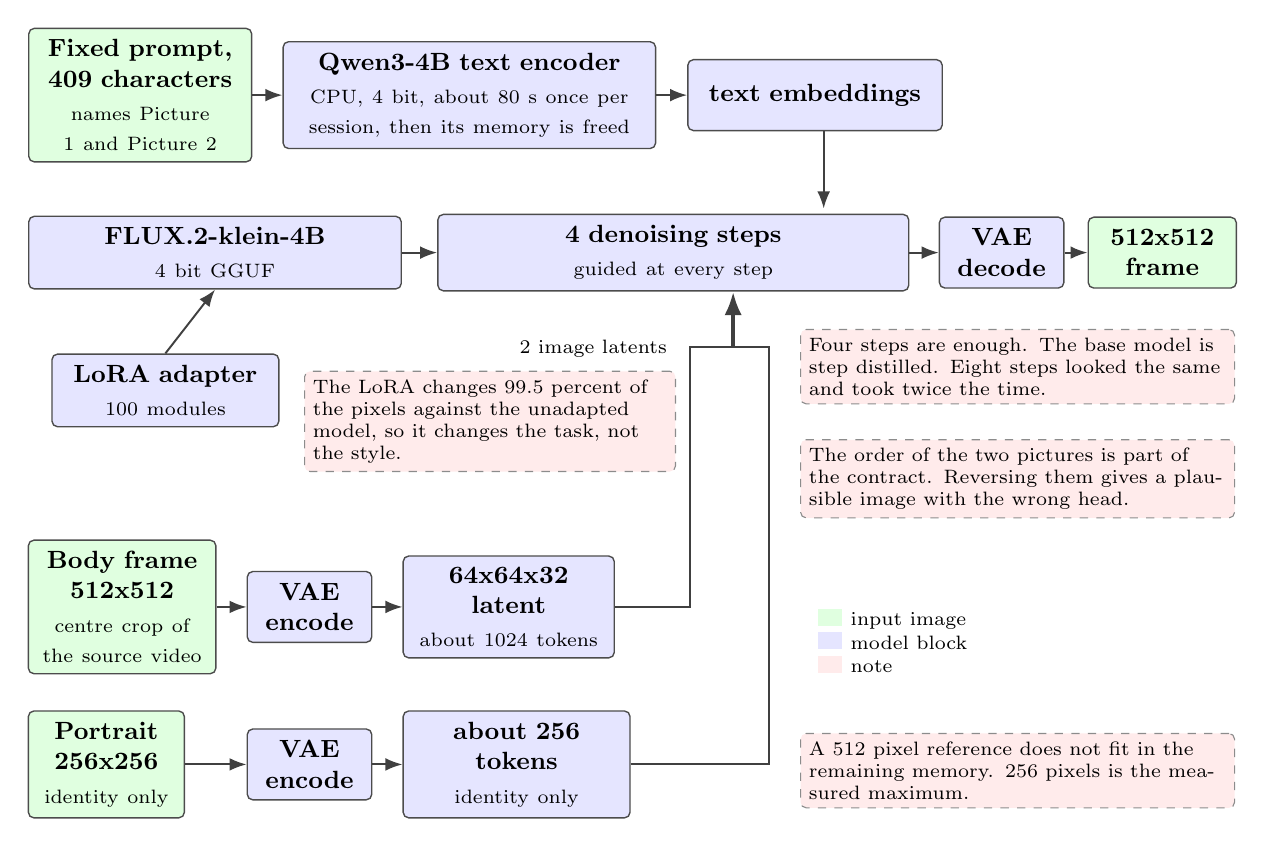
\begin{tikzpicture}[
    x=1cm, y=1cm,
    font=\small,
    block/.style={rectangle, rounded corners=2pt, draw=black!70, line width=0.5pt,
      fill=blue!10, align=center, inner sep=4pt, minimum height=9mm},
    inputblock/.style={rectangle, rounded corners=2pt, draw=black!70, line width=0.5pt,
      fill=green!12, align=center, inner sep=4pt, minimum height=9mm},
    stageblock/.style={rectangle, rounded corners=2pt, draw=black!70, line width=0.5pt,
      fill=orange!15, align=center, inner sep=4pt, minimum height=9mm},
    noteblock/.style={rectangle, rounded corners=2pt, draw=black!45, dashed,
      fill=red!8, align=left, inner sep=3pt, font=\scriptsize},
    flow/.style={->, >=Latex, line width=0.7pt, draw=black!75},
    bundle/.style={->, >=Latex, line width=1.2pt, draw=black!75},
    feed/.style={line width=0.7pt, draw=black!75},
    arrowlab/.style={font=\scriptsize, fill=white, inner sep=1pt},
  ]

  % ---------------- conditioning (top) ----------------
  \node[inputblock, text width=2.55cm] (prompt) at (1.42,4.10)
    {\textbf{Fixed prompt,}\\\textbf{409 characters}\\[1pt]\scriptsize names Picture 1
     and Picture 2};
  \node[block, text width=4.45cm] (enc) at (5.60,4.10)
    {\textbf{Qwen3-4B text encoder}\\[1pt]\scriptsize CPU, 4 bit, about 80 s once per
     session, then its memory is freed};
  \node[block, text width=2.95cm] (emb) at (9.99,4.10) {\textbf{text embeddings}};
  \draw[flow] (prompt.east) -- (enc.west);
  \draw[flow] (enc.east) -- (emb.west);

  % ---------------- denoising chain (middle) ----------------
  \node[block, text width=4.45cm] (flux) at (2.37,2.10)
    {\textbf{FLUX.2-klein-4B}\\[1pt]\scriptsize 4 bit GGUF};
  \node[block, text width=5.70cm] (steps) at (8.19,2.10)
    {\textbf{4 denoising steps}\\[1pt]\scriptsize guided at every step};
  \node[block, text width=1.30cm] (dec) at (12.36,2.10) {\textbf{VAE}\\\textbf{decode}};
  \node[inputblock, text width=1.60cm] (frame) at (14.40,2.10)
    {\textbf{512x512}\\\textbf{frame}};
  \node[block, text width=2.60cm] (lora) at (1.74,0.35)
    {\textbf{LoRA adapter}\\[1pt]\scriptsize 100 modules};
  \draw[flow] (lora.north) -- (flux.south);
  \draw[flow] (flux.east) -- (steps.west);
  \draw[flow] (steps.east) -- (dec.west);
  \draw[flow] (dec.east) -- (frame.west);

  % ---------------- image branches (lower left) ----------------
  \node[inputblock, text width=2.10cm] (bodyf) at (1.19,-2.40)
    {\textbf{Body frame}\\\textbf{512x512}\\[1pt]\scriptsize centre crop of
     the source video};
  \node[block, text width=1.30cm] (vaeA) at (3.57,-2.40) {\textbf{VAE}\\\textbf{encode}};
  \node[block, text width=2.40cm] (latA) at (6.10,-2.40)
    {\textbf{64x64x32 latent}\\[1pt]\scriptsize about 1024 tokens};
  \draw[flow] (bodyf.east) -- (vaeA.west);
  \draw[flow] (vaeA.east) -- (latA.west);

  \node[inputblock, text width=1.70cm] (port) at (0.99,-4.40)
    {\textbf{Portrait}\\\textbf{256x256}\\[1pt]\scriptsize identity only};
  \node[block, text width=1.30cm] (vaeB) at (3.57,-4.40) {\textbf{VAE}\\\textbf{encode}};
  \node[block, text width=2.60cm] (latB) at (6.20,-4.40)
    {\textbf{about 256 tokens}\\[1pt]\scriptsize identity only};
  \draw[flow] (port.east) -- (vaeB.west);
  \draw[flow] (vaeB.east) -- (latB.west);

  % ---------------- conditioning into the denoising steps ----------------
  \draw[flow] (emb.south -| 10.10,0) -- (10.10,2.66);
  \draw[feed] (latA.east) -- (8.40,-2.40) -- (8.40,0.90) -- (8.95,0.90);
  \draw[feed] (latB.east) -- (9.40,-4.40) -- (9.40,0.90) -- (8.95,0.90);
  \draw[bundle] (8.95,0.90) -- (8.95,1.60);
  \node[font=\scriptsize, anchor=east, fill=white, inner sep=1pt] at (8.15,0.88) {2 image latents};

  % ---------------- notes ----------------
  \node[noteblock, text width=4.50cm, anchor=north west] at (3.50,0.60)
    {The LoRA changes 99.5 percent of the pixels against the unadapted model, so it
     changes the task, not the style.};
  \node[noteblock, text width=5.30cm, anchor=north west] at (9.80,1.13)
    {Four steps are enough. The base model is step distilled. Eight steps looked
     the same and took twice the time.};
  \node[noteblock, text width=5.30cm, anchor=north west] at (9.80,-0.27)
    {The order of the two pictures is part of the contract. Reversing them gives a
     plausible image with the wrong head.};
  \node[noteblock, text width=5.30cm, anchor=north west] at (9.80,-4.00)
    {A 512 pixel reference does not fit in the remaining memory. 256 pixels is the
     measured maximum.};

  % ---------------- legend ----------------
  \node[font=\scriptsize, anchor=north west] (leg) at (9.90,-2.30)
    {\begin{tabular}{@{}c@{\hspace{3pt}}l@{}}
       \tikz\fill[draw=black!70,line width=0.4pt,green!12] (0,0) rectangle (0.30,0.20); & input image\\
       \tikz\fill[draw=black!70,line width=0.4pt,blue!10]  (0,0) rectangle (0.30,0.20); & model block\\
       \tikz\fill[draw=black!45,line width=0.4pt,red!8]    (0,0) rectangle (0.30,0.20); & note\\
     \end{tabular}};

  \end{tikzpicture}
  \caption{Inside the generation stage: text conditioning, the image latents, the
    denoiser with its LoRA adapter, and the four denoising steps.}
  \label{fig:generation_architecture}
\end{figure}

\subsubsection{Adapter version comparison}
The recorded clip uses adapter v1 throughout. A newer adapter, v1.1, was released during the work, and we tested two prompt variants, A and B. Table~\ref{tab:adapters} compares the two versions.

v1.1 ran, but it took about 199 seconds per frame against 16.34 for v1. Two measured values rose with it: the adapter rank, from 128 to 512 (four times larger), and the peak allocated memory, from 3.60 GiB to 4.68 GiB, past the 4.0 GiB of the card. That peak value is a PyTorch allocation counter (\texttt{torch.cuda.max\_memory\_allocated}), not driver-level or hardware evidence. Memory pressure is a plausible cause of the slowdown, but the measurements do not settle it. The extra time was not worth it for us.

We judged the look by eye and preferred v1, so the clip kept the v1 output. No metric script was run on v1.1, so every other number here comes from v1. The grids in Figure~\ref{fig:lora_compare} are the only evidence.

\begin{table}[tb]
  \centering
  \footnotesize
  \begin{tabular}{@{}l l l@{}}
    \toprule
    & v1 (recorded) & v1.1 (new) \\
    \midrule
    Adapter rank & 128 & 512 \\
    Seconds per frame & 16.34 & about 199, twelve times slower \\
    Peak VRAM allocated & 3.60 GiB & 4.68 GiB, past the 4.0 GiB of the card \\
    Peak system RAM & 5.48 GiB & 5.3 to 5.5 GiB \\
    Cost for 96 frames & 26 minutes & about 5.3 hours \\
    \bottomrule
  \end{tabular}
  \caption{Adapter v1 against v1.1 on the same machine; only v1 was measured with the metric script.}
  \label{tab:adapters}
\end{table}

\begin{figure}[t]
  \centering
  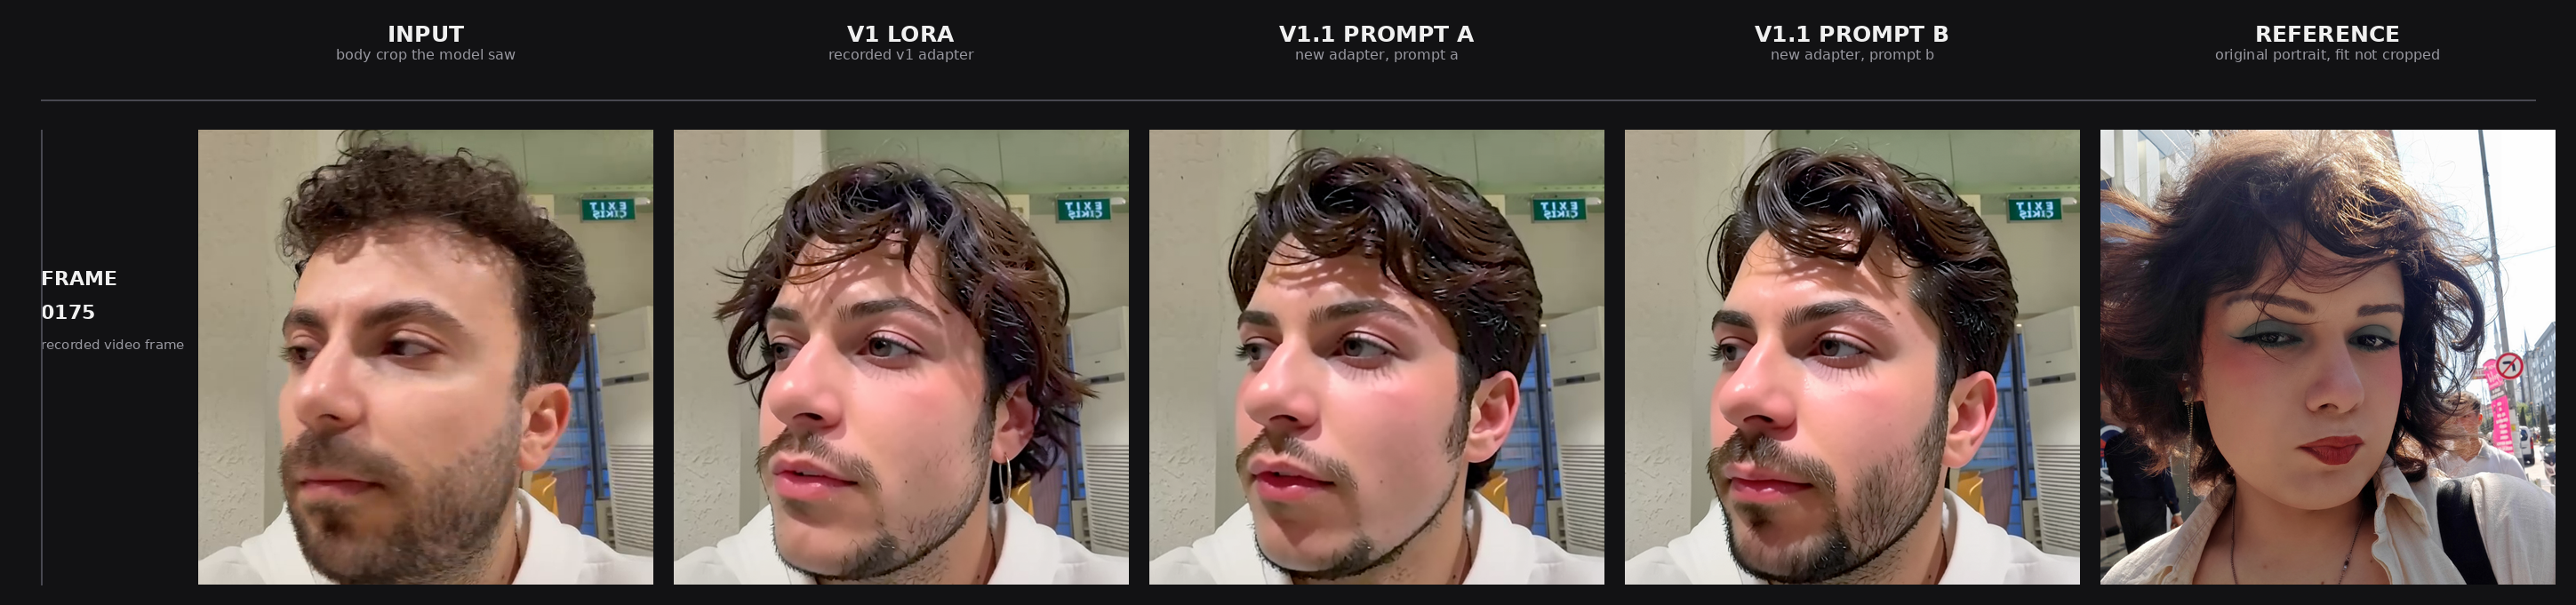
\includegraphics[width=\linewidth]{figures/faceswap_lora_compare_grid_0175.png}\\[3pt]
  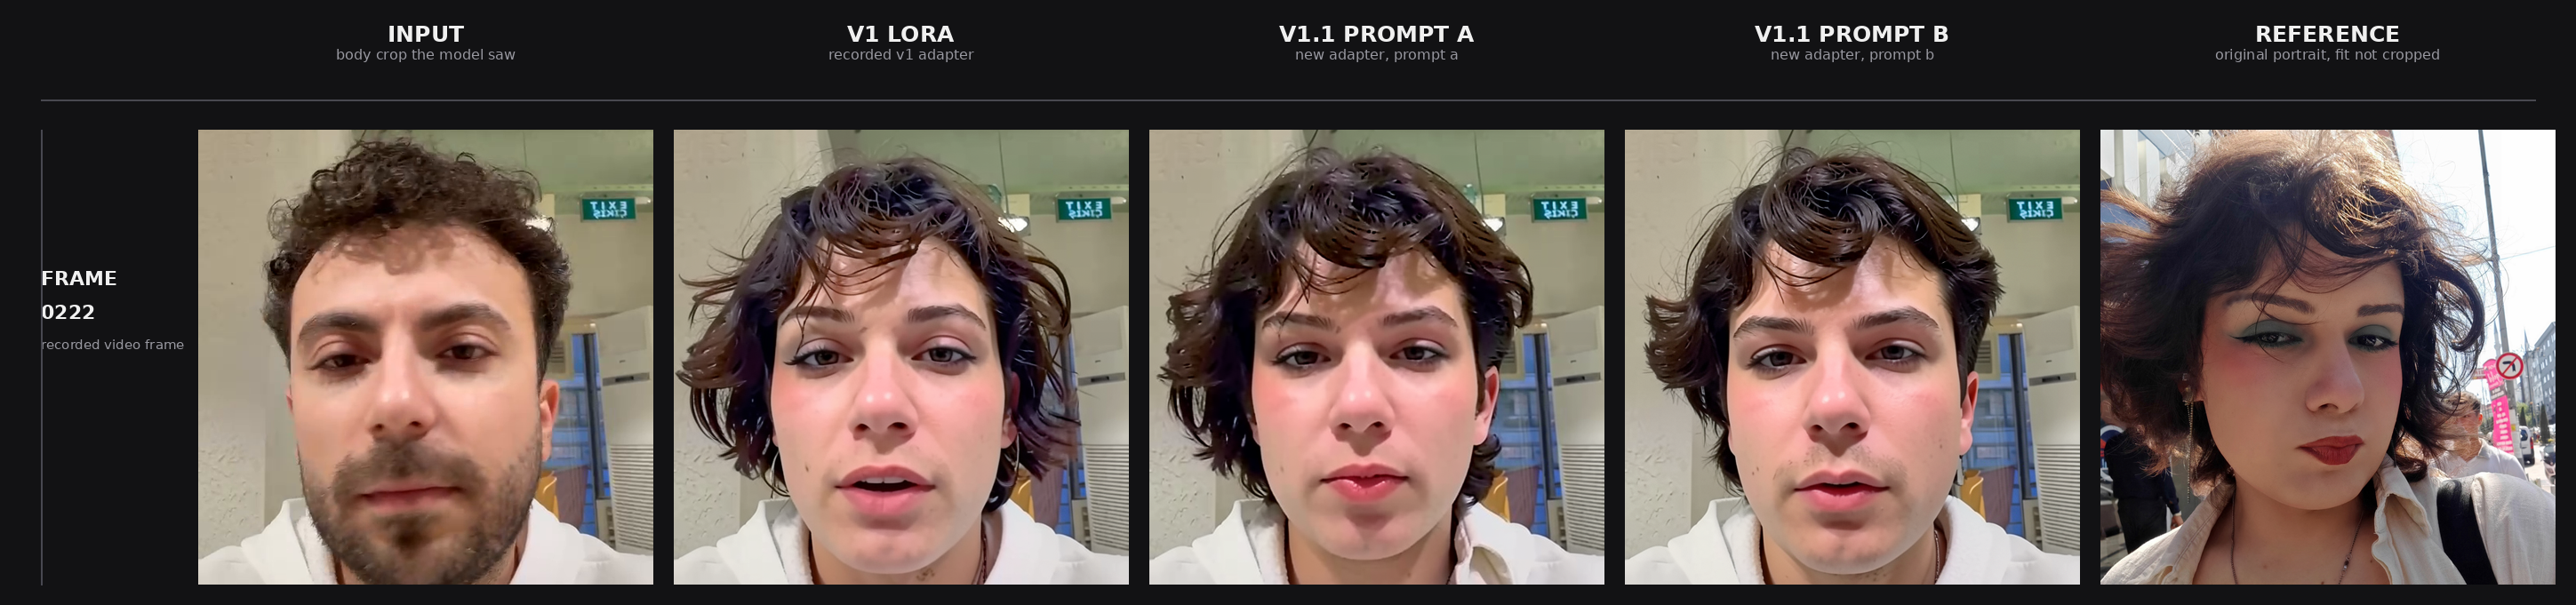
\includegraphics[width=\linewidth]{figures/faceswap_lora_compare_grid_0222.png}\\[3pt]
  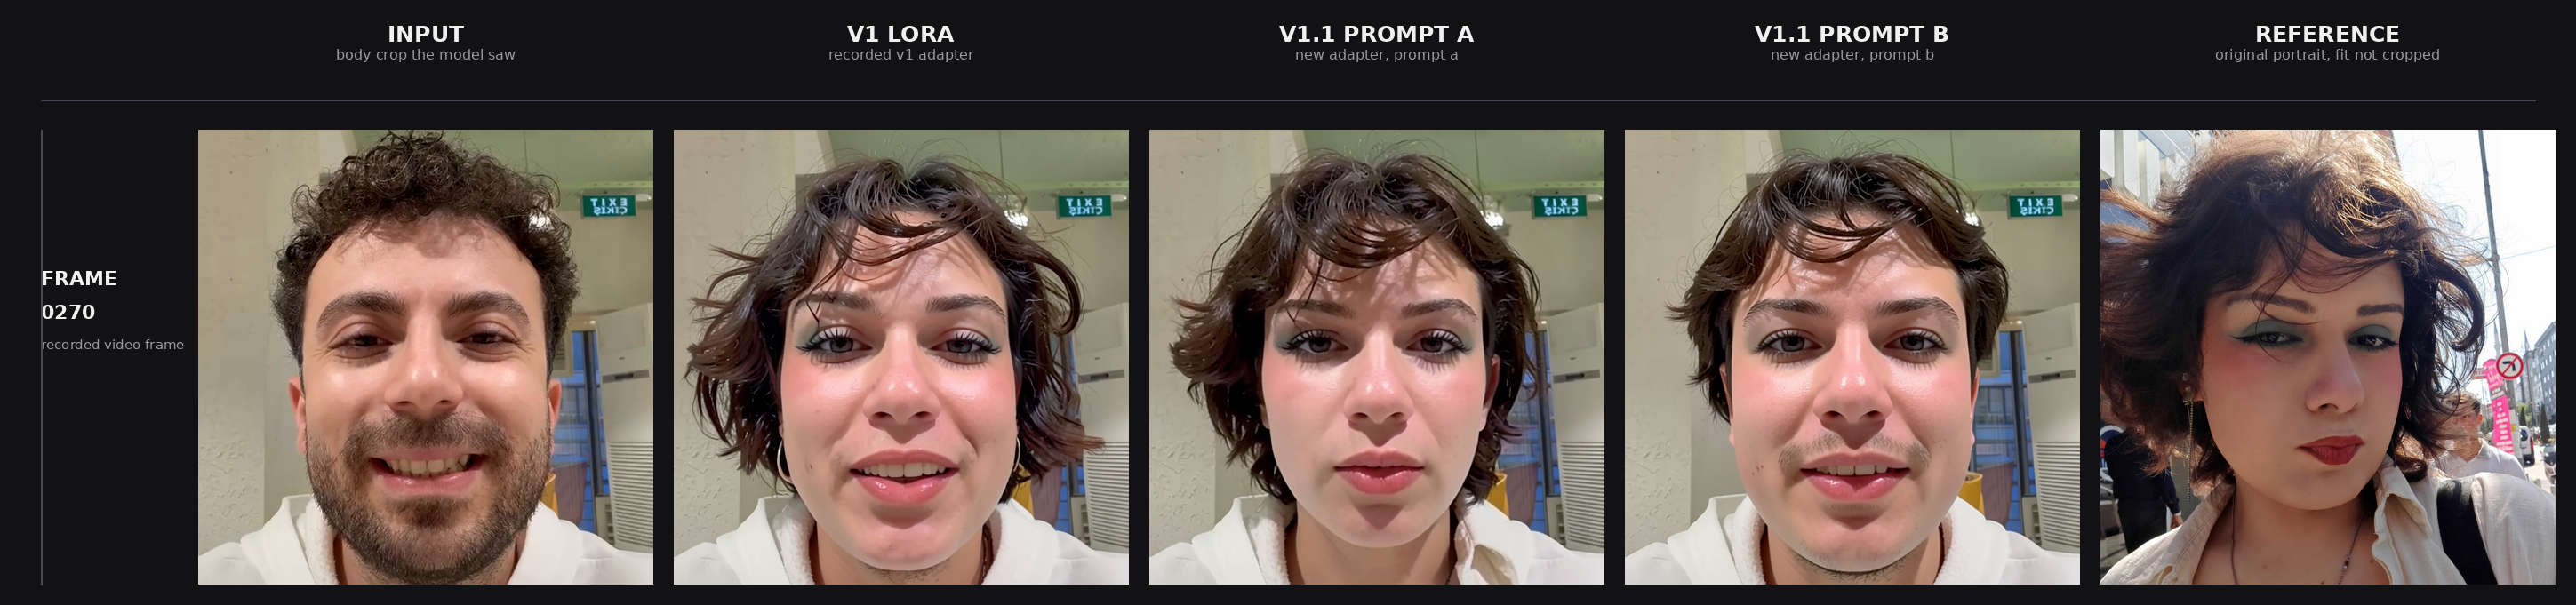
\includegraphics[width=\linewidth]{figures/faceswap_lora_compare_grid_0270.png}
  \caption{Each row is one source frame, the frame number printed inside. The five
  columns run from the input body crop through the v1 adapter, v1.1 with prompt A,
  v1.1 with prompt B, to the reference portrait; only the adapter version and the
  prompt variant change.}
  \label{fig:lora_compare}
\end{figure}

\subsection{Face restoration}
GFPGAN v1.4 cleans every frame (Figure~\ref{fig:restoration}). It detects and aligns the face, runs a restoration network, and composites the crop back. The weights are official, but we built the network in project code because the published wrappers do not import.

The stage costs 0.23 seconds per frame. The frames looked cleaner to us, and the mean face change came down, though the tail improved less.

Hair noise fell slightly, a small gain on its own. The fidelity weight does nothing: the v1.3.4 code passes no weight argument, and newer versions accept it without reading it. Restoration sees one frame at a time, so it does not guarantee temporal consistency.

% Figure: the face restoration stage (detect, align, restore, composite).
% Facts come from diffusion/REPORT.md, section 4.
% Requires in the preamble: \usepackage{tikz} + \usetikzlibrary{positioning,arrows.meta}
\begin{figure}[t]
  \centering
  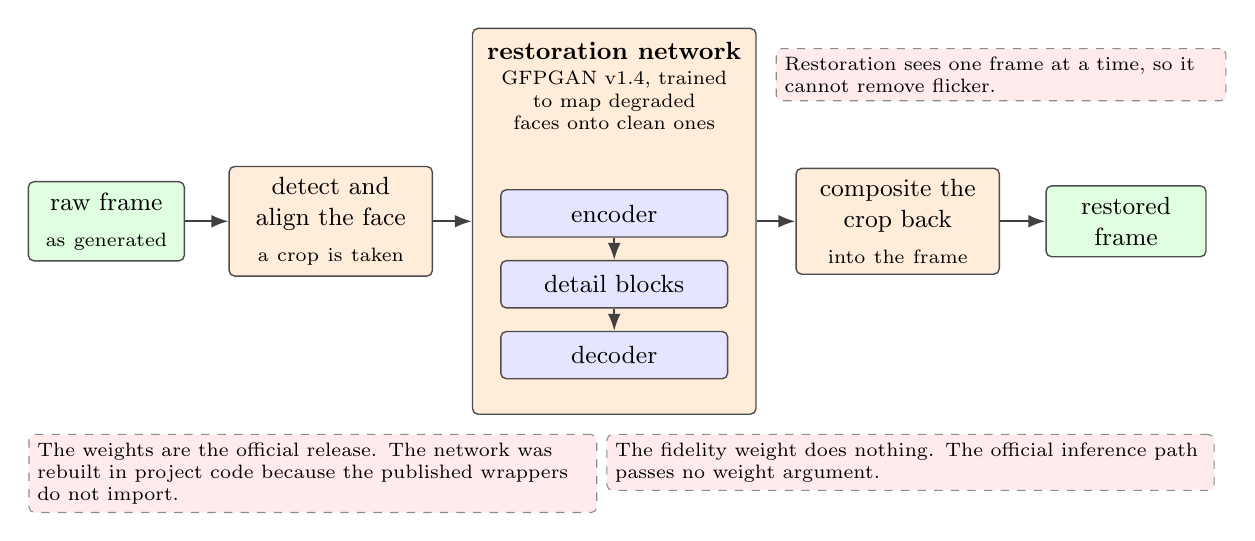
\begin{tikzpicture}[
    x=1cm, y=1cm,
    font=\small,
    block/.style={rectangle, rounded corners=2pt, draw=black!70, line width=0.5pt,
      fill=blue!10, align=center, inner sep=4pt, minimum height=9mm},
    inputblock/.style={block, fill=green!12},
    stageblock/.style={block, fill=orange!15},
    noteblock/.style={rectangle, rounded corners=2pt, draw=black!45, dashed,
      fill=red!8, align=left, inner sep=3pt, font=\scriptsize},
    flow/.style={->, >=Latex, line width=0.7pt, draw=black!75},
    arrowlab/.style={font=\scriptsize, fill=white, inner sep=1pt},
  ]

  % ---------------- main row: frame in, detect and align, restore, composite, frame out
  \node[inputblock, text width=1.70cm] (raw) at (1.10,0)
    {raw frame\\[2pt]{\scriptsize as generated}};
  \node[stageblock, text width=2.30cm] (det) at (3.95,0)
    {detect and\\align the face\\[2pt]{\scriptsize a crop is taken}};

  % the restoration network: one container with a stack of three inner blocks
  \node[stageblock, minimum width=3.60cm, minimum height=4.90cm] (net) at (7.55,0) {};
  \node[anchor=north, inner sep=1pt] (nett) at ([yshift=-4pt]net.north)
    {\textbf{restoration network}};
  \node[anchor=north, inner sep=1pt, font=\scriptsize, text width=3.30cm, align=center]
    (nets) at ([yshift=-2pt]nett.south)
    {GFPGAN v1.4, trained to map degraded faces onto clean ones};
  \node[block, text width=2.60cm, minimum height=6mm] (enc) at (7.55,0.10) {encoder};
  \node[block, text width=2.60cm, minimum height=6mm] (dbl) at (7.55,-0.80) {detail blocks};
  \node[block, text width=2.60cm, minimum height=6mm] (dec) at (7.55,-1.70) {decoder};
  \draw[flow] (enc.south) -- (dbl.north);
  \draw[flow] (dbl.south) -- (dec.north);

  \node[stageblock, text width=2.30cm] (comp) at (11.15,0)
    {composite the\\crop back\\[2pt]{\scriptsize into the frame}};
  \node[inputblock, text width=1.75cm] (res) at (14.05,0)
    {restored\\frame};

  \draw[flow] (raw) -- (det);
  \draw[flow] (det) -- (net);
  \draw[flow] (net) -- (comp);
  \draw[flow] (comp) -- (res);

  % ---------------- notes ----------------
  \node[noteblock, execute at begin node=\raggedright, text width=7.00cm, anchor=north west] at (0.11,-2.70)
    {The weights are the official release. The network was rebuilt in project code
     because the published wrappers do not import.};
  \node[noteblock, execute at begin node=\raggedright, text width=7.50cm, anchor=north west] at (7.45,-2.70)
    {The fidelity weight does nothing. The official inference path passes no weight
     argument.};
  \node[noteblock, execute at begin node=\raggedright, text width=5.50cm, anchor=north west] at (9.60,2.20)
    {Restoration sees one frame at a time, so it cannot remove flicker.};

  \end{tikzpicture}
  \caption{The face restoration stage. Each raw frame is taken on its own: the face is
    detected and aligned, a crop runs through the restoration network, and the restored
    crop is composited back into the frame.}
  \label{fig:restoration}
\end{figure}

\subsection{Temporal smoothing}
The smoothing stage compares frames with each other and removes the boil (Figure~\ref{fig:smoothing}). The per-pixel deflicker averages each pixel with its temporal neighbours, and it is too strong. It costs 0.007 seconds per frame.

The deflicker pushes the face change below the unswapped level. The value has no calibrated threshold, and motion, lighting, texture change and flicker all enter it, so this drop alone does not show that real motion went away. Optical flow estimates the dense motion between neighbouring frames and warps them onto the current one. The warp follows surface points across time, but optical flow does not guarantee temporal consistency. It costs 0.036 seconds per frame.

The control sets the reference change level at 6.66, and the distance column is the face change minus that level. At strength 0.3 the chained pass comes close to the control level, and the raw pass stays above it. A stronger setting sits below the control; the drop cannot separate removed motion from removed flicker.

The recommended output is the chained set at strength 0.3. It beats the flow-only variant on face change, on the tail and on hair noise. Only consecutive identity is slightly lower. The deflicker reaches its low face change at a value below the control; that value cannot separate removed motion from removed flicker, so we kept flow.

\begin{table}[tb]
  \centering
  \footnotesize
  \setlength{\tabcolsep}{4pt}
  \begin{tabular}{@{}l r r r r r r@{}}
    \toprule
    \begin{tabular}[c]{@{}l@{}}Frames\\smoothed\end{tabular} & Strength &
    \begin{tabular}[c]{@{}r@{}}Face\\change\end{tabular} &
    \begin{tabular}[c]{@{}r@{}}Distance from\\the control\end{tabular} & p95 &
    \begin{tabular}[c]{@{}r@{}}Consecutive\\identity\end{tabular} &
    \begin{tabular}[c]{@{}r@{}}Hair\\noise\end{tabular} \\
    \midrule
    Raw & 0.3 & 6.9599 & +0.3034 & 16.2944 & 0.9330 & 32.2358 \\
    Raw & 0.6 & 6.6663 & +0.0098 & 15.6581 & 0.9391 & 32.0603 \\
    Restored, then flow & 0.3 & 6.6303 & -0.0262 & 15.2802 & 0.9377 & 31.7306 \\
    Restored, then flow & 0.6 & 6.3071 & -0.3494 & 14.7575 & 0.9431 & 31.5448 \\
    \bottomrule
  \end{tabular}
  \caption{The smoothing sweep: two frame sets at two strengths, all measured on the same 96 frames.}
  \label{tab:smooth}
\end{table}

% Figure: the temporal smoothing stage (optical flow between neighbouring frames).
% Facts come from diffusion/REPORT.md, section 5.
% Requires in the preamble: \usepackage{tikz} + \usetikzlibrary{positioning,arrows.meta}
\begin{figure}[t]
  \centering
  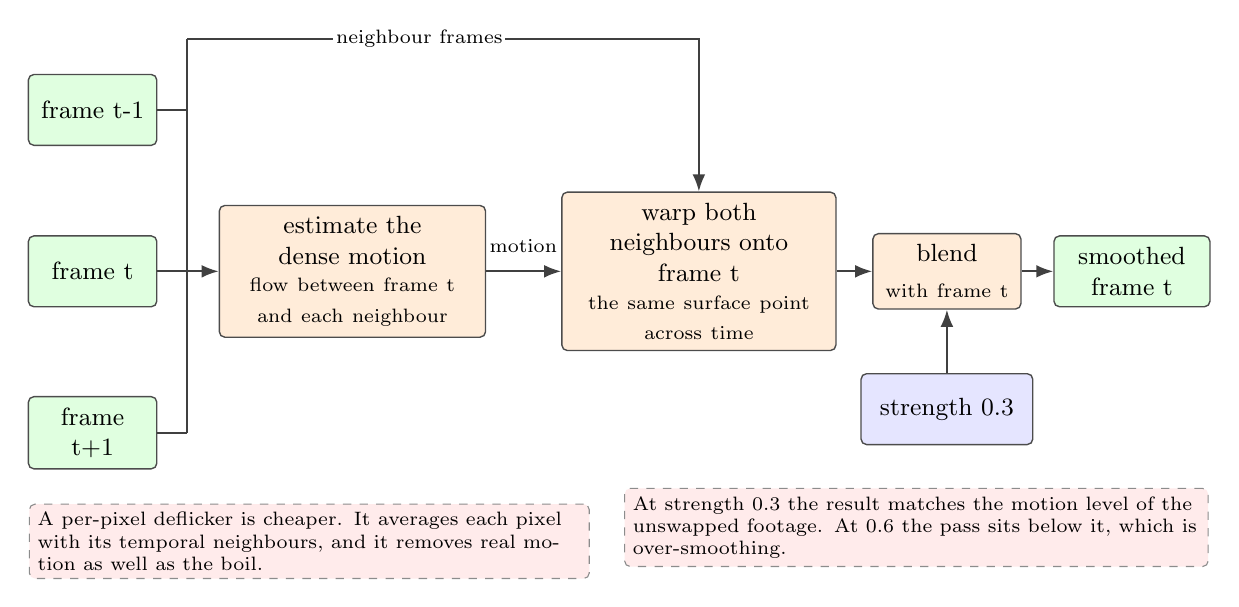
\begin{tikzpicture}[
    x=1cm, y=1cm,
    font=\small,
    block/.style={rectangle, rounded corners=2pt, draw=black!70, line width=0.5pt,
      fill=blue!10, align=center, inner sep=4pt, minimum height=9mm},
    inputblock/.style={block, fill=green!12},
    stageblock/.style={block, fill=orange!15},
    noteblock/.style={rectangle, rounded corners=2pt, draw=black!45, dashed,
      fill=red!8, align=left, inner sep=3pt, font=\scriptsize},
    flow/.style={->, >=Latex, line width=0.7pt, draw=black!75},
    arrowlab/.style={font=\scriptsize, fill=white, inner sep=1pt},
  ]

  % ---------------- three stacked input frames ----------------
  \node[inputblock, text width=1.35cm] (f0) at (1.15,2.05) {frame t-1};
  \node[inputblock, text width=1.35cm] (f1) at (1.15,0.00) {frame t};
  \node[inputblock, text width=1.35cm] (f2) at (1.15,-2.05) {frame t+1};

  % the window of frames enters the stage on one line
  \draw[draw=black!75, line width=0.7pt] (f0.east) -- (2.35,2.05);
  \draw[draw=black!75, line width=0.7pt] (f1.east) -- (2.35,0.00);
  \draw[draw=black!75, line width=0.7pt] (f2.east) -- (2.35,-2.05);
  \draw[draw=black!75, line width=0.7pt] (2.35,-2.05) -- (2.35,2.05);

  % ---------------- main row ----------------
  \node[stageblock, text width=3.10cm] (est) at (4.45,0)
    {estimate the\\dense motion\\[2pt]{\scriptsize flow between frame t\\and each neighbour}};
  \node[stageblock, text width=3.20cm] (warp) at (8.85,0)
    {warp both\\neighbours onto\\frame t\\[2pt]{\scriptsize the same surface point\\across time}};
  \node[stageblock, text width=1.60cm] (blend) at (12.00,0)
    {blend\\[2pt]{\scriptsize with frame t}};
  \node[inputblock, text width=1.70cm] (out) at (14.35,0)
    {smoothed\\frame t};

  \draw[flow] (2.35,0) -- (est.west);
  \draw[flow] (est.east) -- (warp.west);
  \node[arrowlab, anchor=south] at (6.62,0.20) {motion};
  \draw[flow] (warp.east) -- (blend.west);
  \draw[flow] (blend.east) -- (out.west);

  % the two neighbours also reach the warp
  \draw[draw=black!75, line width=0.7pt] (2.35,2.05) -- (2.35,2.95);
  \draw[flow] (2.35,2.95) -- (8.85,2.95) -- (warp.north);
  \node[arrowlab] at (5.30,2.95) {neighbour frames};

  % ---------------- strength input to the blend ----------------
  \node[block, text width=1.90cm] (str) at (12.00,-1.75) {strength 0.3};
  \draw[flow] (str.north) -- (blend.south);

  % ---------------- notes ----------------
  \node[noteblock, text width=6.90cm, anchor=north west] at (0.34,-2.95)
    {A per-pixel deflicker is cheaper. It averages each pixel with its temporal
     neighbours, and it removes real motion as well as the boil.};
  \node[noteblock, text width=7.20cm, anchor=north west] at (7.90,-2.75)
    {At strength 0.3 the result matches the motion level of the unswapped footage.
     At 0.6 the pass sits below it, which is over-smoothing.};

  \end{tikzpicture}
  \caption{The temporal smoothing stage. Each frame is compared with its two
    neighbours: the dense motion is estimated, the neighbours are warped onto frame t
    and the three are blended at strength 0.3.}
  \label{fig:smoothing}
\end{figure}

\subsection{Reassembly}
The encoder turns a frame set into a playable clip (Figure~\ref{fig:reassembly}). It writes H.264 at 29.969 fps and trims both streams. The audio must come from the same interval as the frames, 5.8 to 9.0 seconds of the source. The reassembly tool derives that start from the frame constants, so a normal run takes the audio from 5.839 seconds, and \texttt{-{}-audio-start} overrides it. An earlier version took the full-video audio from t=0, which mixed the wrong interval into the picture. The \texttt{-shortest} flag only cuts the audio to the video length; it does not shift the start. Its output is a 512x512 clip of 3.203 seconds.

The encode is lossy: it changes pixels slightly, but it cannot alter the face motion. In the raw swapped set the face boils, and the results table holds the values.

% Figure: the reassembly stage (encode the frames, mux the source audio back).
% Facts come from rectified_flow/final_report/REPORT.md, section 6.
% Requires in the preamble: \usepackage{tikz} + \usetikzlibrary{positioning,arrows.meta}
\begin{figure}[t]
  \centering
  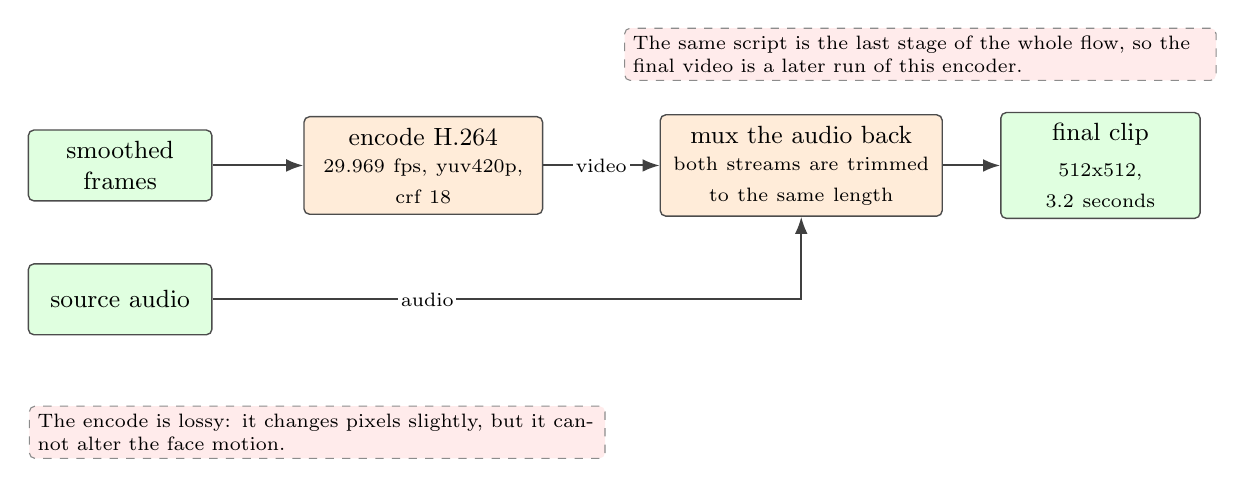
\begin{tikzpicture}[
    x=1cm, y=1cm,
    font=\small,
    block/.style={rectangle, rounded corners=2pt, draw=black!70, line width=0.5pt,
      fill=blue!10, align=center, inner sep=4pt, minimum height=9mm},
    inputblock/.style={block, fill=green!12},
    stageblock/.style={block, fill=orange!15},
    noteblock/.style={rectangle, rounded corners=2pt, draw=black!45, dashed,
      fill=red!8, align=left, inner sep=3pt, font=\scriptsize},
    flow/.style={->, >=Latex, line width=0.7pt, draw=black!75},
    arrowlab/.style={font=\scriptsize, fill=white, inner sep=1pt},
  ]

  % ---------------- the two inputs ----------------
  \node[inputblock, text width=2.05cm] (vid) at (1.70,0.85) {smoothed frames};
  \node[inputblock, text width=2.05cm] (aud) at (1.70,-0.85) {source audio};

  % ---------------- main row ----------------
  \node[stageblock, text width=2.75cm] (enc) at (5.55,0.85)
    {encode H.264\\[2pt]{\scriptsize 29.969 fps, yuv420p,\\crf 18}};
  \node[stageblock, text width=3.30cm] (mux) at (10.35,0.85)
    {mux the audio back\\[2pt]{\scriptsize both streams are trimmed\\to the same length}};
  \node[inputblock, text width=2.25cm] (out) at (14.15,0.85)
    {final clip\\[2pt]{\scriptsize 512x512, 3.2 seconds}};

  \draw[flow] (vid.east) -- (enc.west);
  \draw[flow] (enc.east) -- (mux.west);
  \node[arrowlab] at (7.81,0.85) {video};
  \draw[flow] (mux.east) -- (out.west);

  % ---------------- the audio path, around the encoder ----------------
  \draw[flow] (aud.east) -- (10.35,-0.85) -- (mux.south);
  \node[arrowlab] at (5.60,-0.85) {audio};

  % ---------------- notes ----------------
  \node[noteblock, text width=7.10cm, anchor=north west] at (0.54,-2.20)
    {The encode is lossy: it changes pixels slightly, but it cannot alter the face
     motion.};
  \node[noteblock, text width=7.30cm, anchor=north west] at (8.10,2.60)
    {The same script is the last stage of the whole flow, so the final video is a
     later run of this encoder.};

  \end{tikzpicture}
  \caption{The reassembly stage. The smoothed frames are encoded as H.264 at the source
    rate and the original audio is muxed back; both streams are trimmed to the same
    length.}
  \label{fig:reassembly}
\end{figure}

\subsection{Results}
All numbers come from one script, run once per variant, each on the same 96 frames (175 to 270). Lower hair noise is better, and higher identity values are better. Face change is a temporal change indicator with no calibrated threshold. A value below the control level shows more change removed than the source holds, but motion, lighting, texture change and flicker all enter the number, so the drop alone does not prove that the smoother removed real motion. The control row is the unswapped source footage.

\begin{table}[tb]
  \centering
  \footnotesize
  \begin{tabular}{@{}l r r r r r@{}}
    \toprule
    Stage & \begin{tabular}[c]{@{}r@{}}Face change\\(mean)\end{tabular} &
    \begin{tabular}[c]{@{}r@{}}Face change\\(p95)\end{tabular} &
    \begin{tabular}[c]{@{}r@{}}Consecutive\\identity\end{tabular} &
    \begin{tabular}[c]{@{}r@{}}Identity to\\the portrait\end{tabular} &
    \begin{tabular}[c]{@{}r@{}}Hair\\noise\end{tabular} \\
    \midrule
    \begin{tabular}[t]{@{}l@{}}Control (unswapped\\source footage)\end{tabular} & 6.6565 & 12.3488 & 0.9852 & $-0.0356$ & 31.5999 \\
    Raw head swap & 7.4510 & 17.3794 & 0.9228 & 0.2153 & 32.5703 \\
    Restoration & 7.1602 & 16.2097 & 0.9273 & 0.2153 & 32.0721 \\
    Flow on the raw frames & 6.6663 & 15.6581 & 0.9391 & 0.2148 & 32.0603 \\
    \begin{tabular}[t]{@{}l@{}}Restoration then flow,\\strength 0.3 (recommended)\end{tabular} & 6.6303 & 15.2802 & 0.9377 & 0.2152 & 31.7306 \\
    Deflicker (alternative) & 5.6269 & 12.6650 & 0.9357 & 0.2106 & 31.8960 \\
    \bottomrule
  \end{tabular}
  \caption{All measured variants on the same 96 frames.}
  \label{tab:results}
\end{table}

The identity-to-portrait value of about 0.215 sits above the control value of $-0.0356$. The unswapped footage scores near zero, and every swapped variant scores positive. The output is closer to the reference portrait, but the measure has no calibrated threshold, so this value alone does not prove identity transfer. Consecutive identity, about 0.938 on the recommended set, measures temporal similarity, and a wrong identity that stays consistent also scores high. The recommended set held up well against the control on the mean values. Figure~\ref{fig:stage_strip} shows the effect of each stage on one frame.

\begin{figure}[t]
  \centering
  \begin{minipage}[b]{3.6cm}
    \centering
    
\includegraphics[width=\linewidth]{figures/faceswap_11_body_frame_0175.png}\\[2pt]
    {\scriptsize body input}
  \end{minipage}\hspace{0.28cm}%
  \begin{minipage}[b]{3.6cm}
    \centering
    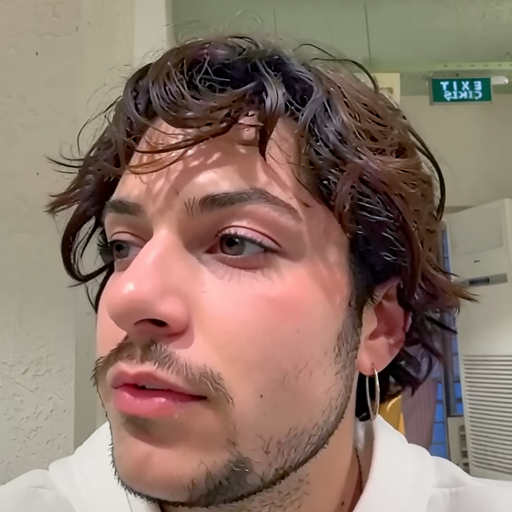
\includegraphics[width=\linewidth]{figures/faceswap_12_raw_head_swap_frame_0175.png}\\[2pt]
    {\scriptsize raw swap}
  \end{minipage}\hspace{0.28cm}%
  \begin{minipage}[b]{3.6cm}
    \centering
    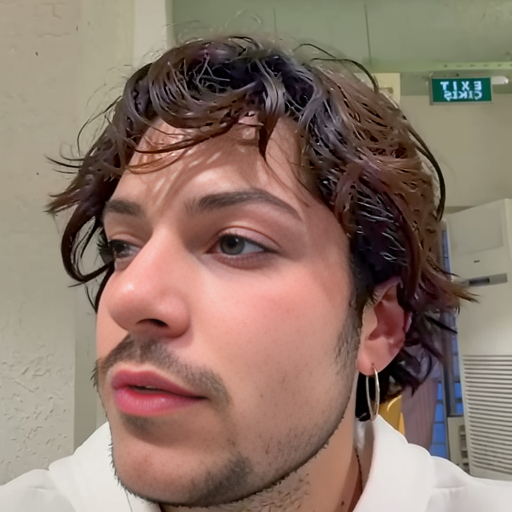
\includegraphics[width=\linewidth]{figures/faceswap_13_restored_frame_0175.png}\\[2pt]
    {\scriptsize after restoration}
  \end{minipage}\hspace{0.28cm}%
  \begin{minipage}[b]{3.6cm}
    \centering
    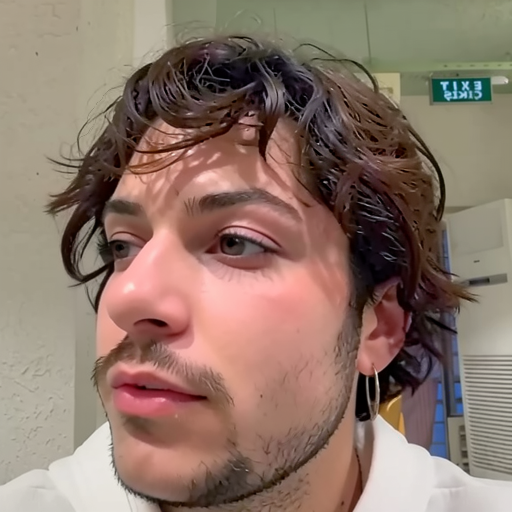
\includegraphics[width=\linewidth]{figures/faceswap_14_smoothed_frame_0175.png}\\[2pt]
    {\scriptsize after smoothing}
  \end{minipage}
  \caption{The same frame 0175 at four points of the flow; the four images are all 512x512.}
  \label{fig:stage_strip}
\end{figure}

\subsection{Problems and decisions}
Attaching the adapter before the first forward pass cost 46 to 48 seconds per frame. Attaching it after one plain pass cost 16 seconds per frame. Peak VRAM was the same in both orders.

We standardised on the fast order. The internal cause was not established, but the effect reproduces exactly and explains an earlier timing discrepancy.

One fixed seed covers the whole clip, so the noise input is constant. The boil still happens, because the model is sensitive to small input changes. Only a pass across frames reduces it.

\subsection{Limits}
The results table shows a mean at the control level, but the tail stays high, so the picture still jumped on some frames. Each step works inside a frame or a short window, so no step removed that tail.

% Section 5: comparison of the three methods.
% Every value comes from Sections 2, 3 and 4; no new measurement.

\section{Comparison}

The three methods attacked the same task from different sides.
Table~\ref{tab:comparison} lists what each one does, what it needs as input, what
it produced in this project, and its main limitation.

\begin{table}[tb]
  \centering
  \footnotesize
  \setlength{\tabcolsep}{4pt}
  \begin{tabular}{@{}p{0.14\textwidth} p{0.25\textwidth} p{0.25\textwidth} p{0.25\textwidth}@{}}
    \toprule
    & \textbf{Autoencoder} & \textbf{FOMM} & \textbf{Rectified flow} \\
    \midrule
    What it does
    & One shared encoder with one decoder per person; a swap means the encoder of one person and the decoder of the other.
    & Animates a source photo with 10 keypoints, one Jacobian per keypoint, a motion field, and an occlusion map.
    & Head swap with a released rectified flow model and a LoRA adapter in four sampling steps, then restoration, smoothing and reassembly. \\
    \midrule
    What it needs
    & 238 prepared face images, 100 of Person A and 138 of Person B, at 128 $\times$ 128.
    & A source portrait of 512 $\times$ 512 and a driving clip of 256 $\times$ 256 with 320 frames at 29.97 FPS.
    & A 256 $\times$ 256 selfie portrait, 512 $\times$ 512 body frames, a fixed prompt of 409 characters, and one laptop with a 4 GB GPU and 8 GB of RAM. \\
    \midrule
    What it produced
    & Both directions (A $\rightarrow$ B and B $\rightarrow$ A) after 50 and 150 epochs. The loss was low, with MSE 0.002935 and 0.001866 at epoch 150, but the output face did not take the other identity. The pretrained FaceFusion models looked better.
    & A 256 $\times$ 256 clip of 320 frames and 10.7 s in about 2.5 minutes on CPU. Head turns and blinks transferred smoothly, but braces disappeared in some frames.
    & A 96-frame 512 $\times$ 512 clip of 3.203 s with the original audio. The identity-to-portrait value was about 0.215 against $-0.0356$ for the control. \\
    \midrule
    Main limitation
    & The reconstruction objective teaches the model to rebuild the input, not to transfer an identity, and the dataset was small.
    & Inpainting falls back on learned appearance priors, so rare personal details are lost and large head turns blur. No state passes from frame to frame.
    & Every frame is generated on its own, so the face boils; smoothing reduces the boil, but the worst frames still jump. \\
    \bottomrule
  \end{tabular}
  \caption{The three methods: what each one does, its input, its result in this
    project, and its main limitation.}
  \label{tab:comparison}
\end{table}

The table shows three different trade-offs. The autoencoder needed our own
training data and still missed the identity transfer, and our own model stayed
behind the pretrained FaceFusion models. FOMM gave a fast per-frame method and
moved head turns and blinks smoothly, but its inpainting lost rare details and
it keeps no memory across frames. The rectified flow pipeline cost 16.3 seconds
per frame in the generation stage, and the worst frames still jump, yet it
produced a full 512 $\times$ 512 clip with the original audio on the hardware we
had. We would recommend that pipeline, with restoration followed by
optical-flow smoothing at strength 0.3. Its identity-to-portrait value stayed
above the control level, and the full clip ran on one laptop with a 4 GB GPU.

% Section 6: ethics and the limits of this project.
% The limitation facts follow a check of this checkout:
%   autoencoders/ holds no training code and no weights;
%   rectified_flow/final_report/ and rectified_flow/out/ are untracked run artifacts,
%   so the raw run records, the metric CSV and the 96-frame sets are not in the repository;
%   no FOMM checkpoint is present (fomm/vox-cpk.pth.tar is ignored and absent);
%   the mean absolute pixel difference helper works on 8-bit pixel values.

\section{Ethics and Limitations}

\subsection{Ethics}
Face reenactment carries a clear risk of misuse. The same pipeline that makes a
light-hearted clip can put a real face on words the person never said, and a
viewer cannot separate the two cases by eye. The risk grows as soon as the
material leaves the team.

We answer that risk with provenance, with watermarks and with detection
research. The technical measures limit what a stranger can do with a published
file.

C2PA is a signed provenance and edit-history manifest. It records which tool
made a file, what changed it and when, and a signature lets a reader check that
record. It is not a stamp that exists only at capture time, because an editor
can add a further manifest entry for each change, and the history then travels
with the file. C2PA is also not a deepfake detector by itself. The manifest
reports where a file came from and how it changed; it does not judge whether the
content is real.

Watermarking is a separate measure. It hides a signal inside the pixels or the
audio, and the signal travels with the content. A watermark and a C2PA manifest
do different jobs, so a project can use both.

Research also reports detection cues. Eye blinking follows a rhythm that the
early face generators did not reproduce (Li et al., 2018). Remote
photoplethysmography reads a heartbeat signal from small colour changes in the
skin (Qi et al., 2020). Frequency analysis finds the traces that neural
upsampling leaves in the image spectrum (Frank et al., 2020). We treat these
cues as research examples only. This project ran no detection experiment and
trained no detector, so we report no measurement of our own here.

\subsection{Limitations}
Our results rest on artifacts that are not all in the repository. The
autoencoder training code and the trained weights are absent, so that training
cannot be repeated from this checkout. The Rectified Flow raw run records, the
metric CSV and the 96-frame sets are absent as well, so the numbers in
Section 4 cannot be re-derived here. The FOMM checkpoint is absent too, so the
training history of those weights cannot be verified; the released
configuration trains no adversarial loss, as Section 3 states.

Two explanations stay unverified. We ran no analysis of the dataset content, so
the braces explanation in Section 3 stays a hypothesis and not a finding. The
temporal metric thresholds are not calibrated, so a face change value has no
absolute reading; only the control level gives it a meaning.

One helper limits what one number can show. The script that reports the mean
absolute difference converts both images to 8-bit pixel values before the
subtraction, an 8-bit round trip. The value therefore cannot show a difference
finer than one 8-bit level.

These limits do not change any measured value. They set the size of each claim
we make, and we report only what the artifacts support.

% Section 7: general conclusion across the three methods.
% No new measurements; the numbers stay in Sections 2 to 5.

\section{Conclusion}

The three methods left us with three different results. FOMM moved head turns
and blinks smoothly and produced its clip in about 2.5 minutes, but it lost rare
details such as braces when it inpainted the mouth. The rectified flow pipeline
produced a 512 $\times$ 512 clip with sound on the 4 GB laptop we had, and its
restoration and smoothing stages removed much of the boil. Our own autoencoder
rebuilt faces well, but it never learned to move an identity from one person to
the other.

The failures had reasons, or at least clear hypotheses. The autoencoder loss
went down while the swap stayed wrong, because the training objective rewarded
reconstruction and our dataset of 238 images was small; 100 more epochs did not
change the result. The lost braces on FOMM have a hypothesis and no direct
evidence: the training videos may show no braces, so the learned appearance
priors cannot rebuild them. In the rectified flow clip every frame is generated
on its own, so the face boils, and the smoothing only works inside short
windows; the worst frames still jump. The newer adapter v1.1 was twelve times
slower than v1, so the recorded clip kept v1.

What we learned reaches past the single results. A low loss does not mean a
usable face swap, so the measure must match the goal. A model built for the
task, even a released checkpoint, gave more than our own simple model. Per-frame
generation always boils, and only a pass across frames reduces it. Finally,
every measure here has limits: the face change value mixes motion, lighting,
texture and flicker, and it has no calibrated threshold, so we read the numbers
together with the frames, not instead of them.

% Section 8: the teamwork record and the meeting evidence.
% The assignment asks for evidence of at least two team meetings.
% Paste the meeting screenshots over the two TODO markers below.
% The example figure block stays commented out until a picture file exists.

\section{Meetings}

We couldn't arrange an in-person meeting so both meetings are held online as listed in Table~\ref{tab:meetings}.

\begin{table}[tb]
  \centering
  \footnotesize
  \setlength{\tabcolsep}{4pt}
  \begin{tabular}{@{}c p{0.11\textwidth} p{0.15\textwidth}
                    p{0.20\textwidth} p{0.36\textwidth}@{}}
    \toprule
    No. & Date & Mode & Attendees & Decisions \\
    \midrule
    1 & \textbf{3.10.2026} & \textbf{Online}
    & \textbf{Yusuf, Erdem, Mehmet}
    & \textbf{Yusuf, Erdem and Mehmet works on GAN, Autoencoder and Diffusion respectively.} \\
    2 & \textbf{10.10.2026} & \textbf{Online}
    & \textbf{Yusuf, Erdem, Mehmet and Eren}
    & \textbf{Discussion of findings and division of tasks for report and presentation creation.} \\
    \bottomrule
  \end{tabular}
  \caption{The team meetings.}
  \label{tab:meetings}
\end{table}

\begin{center}
  \fbox{\parbox{0.92\textwidth}{\centering \textbf{
    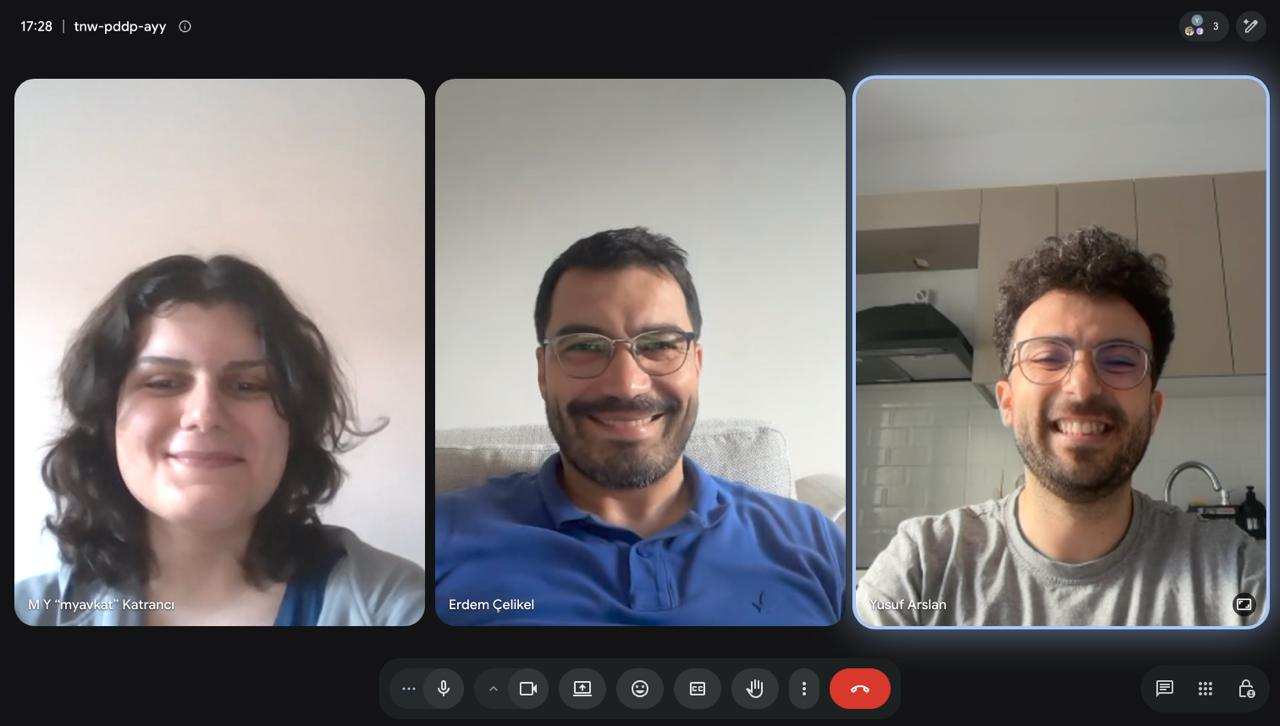
\includegraphics[width=0.85\textwidth]{figures/Toplanti1.jpeg}
    \captionof{figure}{The first team meeting.}
    \label{fig:meeting1}
  }}}
\end{center}

\medskip

\begin{center}
  \fbox{\parbox{0.92\textwidth}{\centering \textbf{
    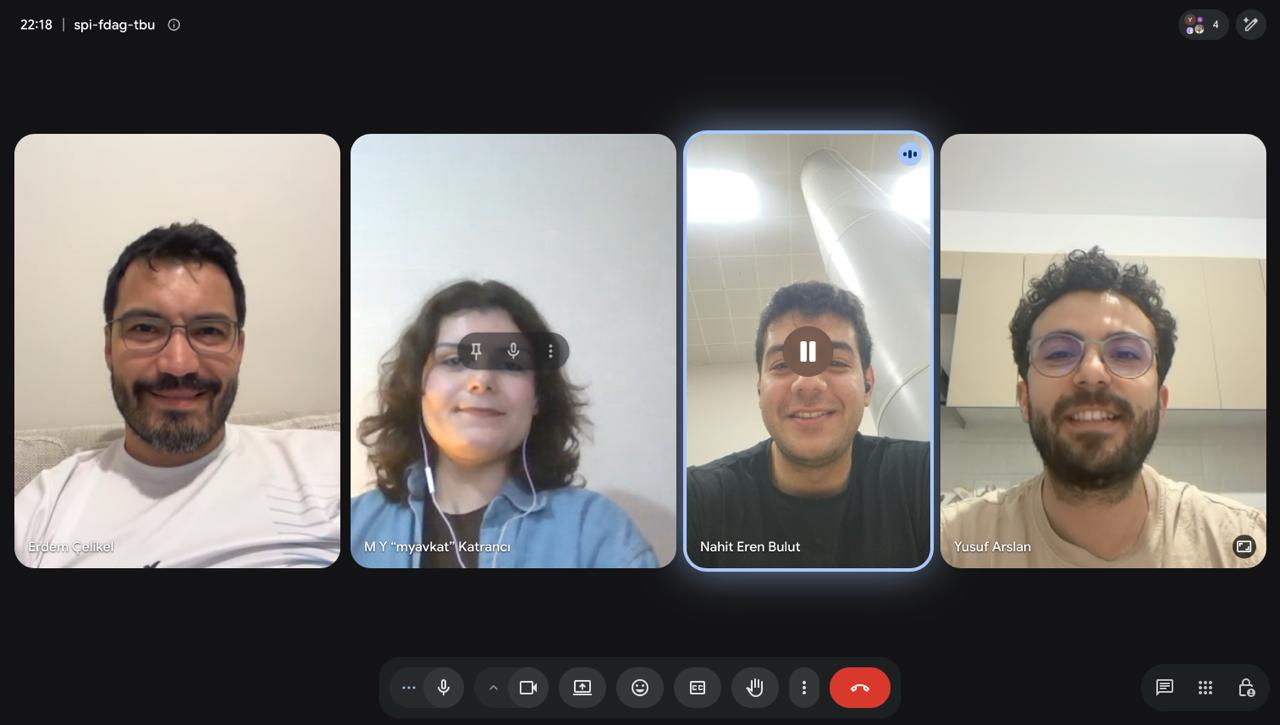
\includegraphics[width=0.85\textwidth]{figures/Toplanti2.jpeg}
    \captionof{figure}{The second team meeting.}
    \label{fig:meeting2}
  }}}
\end{center}

% When a picture is ready, uncomment and adjust this example block:
% \begin{figure}[tb]
%   \centering
%   \includegraphics[width=0.85\textwidth]{figures/meeting_1.png}
%   \caption{The first team meeting.}
%   \label{fig:meeting1}
% \end{figure}

The team divided the work by method, and each member wrote the part of the
report that covers that method. \textbf{Erdem} built and trained
the autoencoder, \textbf{Yusuf} ran the FOMM experiment,
\textbf{Mehmet} ran the rectified flow pipeline, and
\textbf{Eren} wrote the shared chapters and the slides.


% Report content will be added here

% The reference list reads docs/report/references.bib.
% It is disabled at the author's request: the chapters name their sources in
% the text instead. The .bib file stays on disk for a later switch back.
% \nocite{*}
% \bibliographystyle{plain}
% \bibliography{references}

\end{document}

